\documentclass[11pt,a4paper]{article}
\usepackage[utf8]{inputenc}
\usepackage[english]{babel}
\usepackage{amsmath}
\usepackage{amsfonts}
\usepackage{amssymb}
\usepackage{graphicx}
\usepackage{auto-pst-pdf}
\usepackage{pstricks}
\usepackage{paralist}
\usepackage{float}
\usepackage{tabularx}
\usepackage{subcaption}
\usepackage{hyperref}
\usepackage[left=2cm,right=2cm,top=2cm,bottom=2cm]{geometry}
\numberwithin{equation}{section}
\numberwithin{figure}{section}
\setlength{\parindent}{0pt}
\usepackage{titlesec}
\setcounter{secnumdepth}{4}
\titleformat{\paragraph}
{\normalfont\normalsize\bfseries}{\theparagraph}{1em}{}
\titlespacing*{\paragraph}
{0pt}{3.25ex plus 1ex minus .2ex}{1.5ex plus .2ex}
\title{GEOEEM WS 15/16}
\author{Lecturer: B. Tezkan}
\begin{document}

\newcommand{\tens}[1]{\underline{\underline{#1}}}

\graphicspath{ {figs/} }

\begin{titlepage}
\maketitle
\thispagestyle{empty}
\end{titlepage}
\newpage
\tableofcontents
\newpage

%\section*{DC resistivity and electromagnetic methods}
\setcounter{section}{-1}
\section{Introduction}
Common to each method is the fact that the current flow is used in the subsurface. The aim is the determination of the conductivity distribution of the subsurface from the Earth's surface down to several 100 km depth.

Application areas:
\begin{itemize}
\item Near surface exploration (0 - 300 m depth): 
\begin{itemize}
\item Application for the environment: Waste site exploration, search for suitable landfill sites, ...
\item Groundwater exploration
\item Archaeology
\item Exploration for deposits, engineering applications (e.g. cativity detection,...)
\end{itemize}
\item Exploration of deep structures ( $>$ 300 m)
\begin{itemize}
\item Geothermal fields, oil and gas exploration
\item tectonic questions, shear zones
\item deep crust and upper mantle
\end{itemize}


\end{itemize}
\subsection{Classification of methods}
Classifications possible as:
\begin{itemize}
\item According to the source (artificial or natural)
\item Inclusion of magnetic field or not?
\item Direct current or alternating current?
\end{itemize}
\begin{description}
\item[DC-resistivity methods:] Direct current resistivity (DC), Induced polarization (IP), Self potential (SP)
\item[Electromagnetic methods:] ~\\
\begin{itemize}
\item \textit{Frequency domain}: Magnetotellurics (MT), Audiomagnetotellurics (AMT), Controlled source AMT (CSAMT), Radiomagnetotellurics (RMT)
\item \textit{Time domain:} Transient electromagnetics (TEM), Long offset transient electromagnetics (LOTEM)
\end{itemize}
\item[Electromagnetic methods using high frequencies ($f > 10$ MHz):] Ground penetrating radar (GPR)
\end{description}


\section{Conductivity}

The conductivity $\sigma$ of the minerals in the nature covers a range of 25 decades! For example:
\begin{align*}
10^{-18} S/m &\rightarrow \textrm{Diamand}\\
10^{7} S/m &\rightarrow \textrm{Copper}\\
\end{align*}
Instead of the conductivity, the resistivity $\rho=\frac{1}{\sigma} \Omega m$ is often used.

\subsubsection*{Definition: Ohm's law}
Let us consider a rock sample of length $L$, resistivity $\rho$ and cross section $A$.
\begin{figure}[h!]
\begin{center}
\resizebox{0.4\textwidth}{!}
{
\begin{pspicture}(0,-2.5217187)(8.62,2.5217187)
\psellipse[linewidth=0.04,dimen=outer](1.2,-0.58171874)(0.6,1.0)
\psline[linewidth=0.04cm](1.2,0.41828126)(7.6,0.41828126)
\psline[linewidth=0.04cm](1.3,-1.5817188)(7.6,-1.5817188)
\psbezier[linewidth=0.04](7.6,-1.5817188)(8.1,-1.0817188)(8.1,-0.08171875)(7.6,0.41828126)
\psline[linewidth=0.04cm](8.0,-0.58171874)(8.6,-0.58171874)
\psline[linewidth=0.04cm](8.6,-0.58171874)(8.6,1.4182812)
\psline[linewidth=0.04cm](8.6,1.4182812)(4.9,1.4182812)
\psline[linewidth=0.04cm](4.3,1.4182812)(0.0,1.4182812)
\psline[linewidth=0.04cm](0.0,1.4182812)(0.0,-0.58171874)
\psline[linewidth=0.04cm](0.0,-0.58171874)(0.9,-0.58171874)
\usefont{T1}{ptm}{m}{n}
\rput(1.2460938,-0.57171875){\huge A}
\usefont{T1}{ptm}{m}{n}
\rput(4.1992188,-0.57171875){\huge I}
\usefont{T1}{ptm}{m}{n}
\rput(5.4471874,2.2282813){\huge U}
\usefont{T1}{ptm}{m}{n}
\rput(4.3992186,-2.2717187){\huge L}
\pscircle[linewidth=0.04,dimen=outer](4.6,1.4182812){0.3}
\psline[linewidth=0.04cm,arrowsize=0.05291667cm 2.0,arrowlength=1.4,arrowinset=0.4]{->}(4.7,-2.2817187)(7.6,-2.2817187)
\psline[linewidth=0.04cm,arrowsize=0.05291667cm 2.0,arrowlength=1.4,arrowinset=0.4]{->}(4.1,-2.2817187)(1.2,-2.2817187)
\end{pspicture} 
}

\caption{Schematic derivation of Ohm's law}
\label{fig:ohmslaw}
\end{center}
\end{figure}

A current $I [A]$ flows by applying a voltag $U [V]$ to the rock sample:

\begin{align*}
I&=\frac{AU}{\rho L}\\
\Leftrightarrow \rho\underbrace{\frac{I}{A}}_{\textrm{current density }j}&=\underbrace{\frac{U}{L}}_{\textrm{electric Field }E}
\end{align*}
\begin{equation}
\vec{j}\rho=\vec{E}\label{eq:1-2}
\end{equation}
We measure $I$ and $U$, $A$ and $L$ are known, so we can calculate $\rho$.

\subsection{Mechanisms of electrical conductivity}
\begin{description}
\item[Metallic conductivity:] Current flows by free electrons $\rho\equiv T$
\item[Electrolytic conductivity:] Charge carriers are cations and anions: $\rho$ decreases with temperature $T$.
\item[Semi-conductors:] Charge carriers must be activated by heat, light or EM-radiation. Strongly dependent on temperature $T$. Important for mantle (deep earth structures)
\item[Boundary layer conductivity:] Occurs due to the interaction of the pore liquid with the rock matrix. This is the source of SP-anomalies!
\end{description}


\section{DC-resistivity method}

\begin{figure}[H]
\begin{center}
\resizebox{0.5\textwidth}{!}
{
\begin{pspicture}(0,-2.0159376)(15.188437,2.0159376)
\psline[linewidth=0.04cm](0.1684375,-1.0303125)(15.168438,-1.0303125)
\psline[linewidth=0.04cm,arrowsize=0.05291667cm 2.0,arrowlength=1.4,arrowinset=0.4]{->}(3.1684375,0.9696875)(3.1684375,-1.0303125)
\psline[linewidth=0.04cm,arrowsize=0.05291667cm 2.0,arrowlength=1.4,arrowinset=0.4]{->}(6.1684375,-0.0303125)(6.1684375,-1.0303125)
\psline[linewidth=0.04cm,arrowsize=0.05291667cm 2.0,arrowlength=1.4,arrowinset=0.4]{->}(9.168438,-0.0303125)(9.168438,-1.0303125)
\psline[linewidth=0.04cm,arrowsize=0.05291667cm 2.0,arrowlength=1.4,arrowinset=0.4]{->}(12.168438,0.9696875)(12.168438,-1.0303125)
\psline[linewidth=0.04cm](6.1684375,-0.0303125)(7.4684377,-0.0303125)
\psline[linewidth=0.04cm](7.9684377,-0.0303125)(9.168438,-0.0303125)
\psline[linewidth=0.04cm](3.1684375,0.9696875)(8.168438,0.9696875)
\psline[linewidth=0.04cm](9.168438,0.9696875)(12.168438,0.9696875)
\pscircle[linewidth=0.04,dimen=outer](7.7184377,0.0196875){0.25}
\pscircle[linewidth=0.04,dimen=outer](8.668438,0.9696875){0.5}
\psline[linewidth=0.04cm,arrowsize=0.05291667cm 2.0,arrowlength=1.4,arrowinset=0.4]{->}(7.4684377,-0.2303125)(8.068438,0.3696875)
\psline[linewidth=0.04cm,arrowsize=0.05291667cm 2.0,arrowlength=1.4,arrowinset=0.4]{->}(8.168438,0.4696875)(9.268437,1.6696875)
\usefont{T1}{ptm}{m}{n}
\rput(7.9475,-0.4553125){\LARGE $\Delta U$}
\usefont{T1}{ptm}{m}{n}
\rput(7.974375,1.7446876){\LARGE Source $I$}
\usefont{T1}{ptm}{m}{n}
\rput(3.179375,-1.4553125){\LARGE A}
\usefont{T1}{ptm}{m}{n}
\rput(6.223906,-1.4553125){\LARGE M}
\usefont{T1}{ptm}{m}{n}
\rput(9.084687,-1.4553125){\LARGE N}
\usefont{T1}{ptm}{m}{n}
\rput(12.147187,-1.4553125){\LARGE B}
\usefont{T1}{ptm}{m}{n}
\rput(1.4175,-1.7553124){\LARGE $\rho$}
\usefont{T1}{ptm}{m}{n}
\rput(1.5075,-0.4553125){\LARGE $\rho=\infty$}
\end{pspicture} 
}

\caption{Four point measurement}
\label{fig:dc01}
\end{center}
\end{figure}
Resistivity $\rho$ of the subsurface derived from $I$ (which is known), $\Delta U$ (which is measured) and the geometrical factor $K$ (which is also known).

\subsubsection*{Frequently used electrode arrays}

\begin{figure}[H]
\begin{center}
\includegraphics[width=0.5\textwidth]{Wenner.png}
a)
\includegraphics[width=0.5\textwidth]{Schlumberger.png}
b)
\includegraphics[width=0.5\textwidth]{Dipoldipol.png}
c)
\caption{a) Wenner, Half-Wenner; b) Schlumberger, Half-Schlumberger; c) Dipole-dipole, source???}
\label{fig:dc02}
\end{center}
\end{figure}

Industrial standard of measuring is via an \textit{Multielectrode array}.


\subsection{Basic equations of DC-resistivity}
The first assumption of DC-resistivity methods and the major difference to EM-methods is the assumption of stationary currents:
\begin{align*}
\frac{\partial}{\partial t}=0
\end{align*}
The fields do not depend on time.

Looking at the \textit{Maxwell's equations}:
\begin{align}
\nabla\times\vec{E}=\frac{\partial \vec{B}}{\partial t}=0
\end{align}
This means irrotational electric field and from that follows, that the electric field vector can be derived by a scalar potential:

\begin{equation}
\vec{E}=-\nabla V \label{eq:2-2}
\end{equation}
Insert equation \eqref{eq:2-2} into eq. \eqref{eq:1-2}:

\begin{equation}
\vec{j}=-\sigma \nabla V\label{eq:2-3}
\end{equation}
\textit{Continuity equation:}
\begin{equation}
\nabla\cdot\vec{j}+\frac{\partial q}{\partial t}=0
\end{equation}
Now new charges are generated in the course of time
\begin{equation}
\nabla\cdot\vec{j}=0 \label{eq:2-5}
\end{equation}
which is valid outside of the source.

If we insert eq. \eqref{eq:2-3} into \eqref{eq:2-5}:
\begin{align*}
-\nabla\cdot(\sigma\nabla V)&=0\\
\nabla\sigma\nabla V + \sigma\nabla^2V&=0
\end{align*}
$\nabla\sigma=0$ for areas with constant conductivity, so:
\begin{equation}
\nabla^2 V=0\label{eq:lapleq}
\end{equation}
which is called the \textit{Laplace-equation}, the basic equation of DC-resistivity.

Derivation of solutions of this elliptic partial differential equation using  different boundary conditions:

Assume a current source with strength $I$ at point $\vec{r}_0$, then the spatial current distribution can be given as:$\nabla\cdot\vec{j}=I\delta(\vec{r}-\vec{r}_0$
and so:
\begin{equation}
\nabla\cdot(\sigma\nabla V)=-I\delta(\vec{r}-\vec{r}_0)
\end{equation}
This equation can be solved numerically for arbitrary distribution of conductivity ratio.


\subsubsection{Potential of a current electrode}

\begin{figure}[H]
\begin{center}
\resizebox{0.5\textwidth}{!}
{
\begin{pspicture}(0,-3.02)(10.189688,1.02)
\psline[linewidth=0.04cm](0.0,0.0)(8.0,0.0)
\rput{-180.0}(8.0,0.0){\psarc[linewidth=0.04,linestyle=dashed,dash=0.16cm 0.16cm](4.0,0.0){3.0}{0.0}{180.0}}
\psline[linewidth=0.04cm,arrowsize=0.05291667cm 2.0,arrowlength=1.4,arrowinset=0.4]{->}(4.0,1.0)(4.0,0.0)
\psline[linewidth=0.04cm,arrowsize=0.05291667cm 2.0,arrowlength=1.4,arrowinset=0.4]{->}(4.0,0.0)(1.2,-1.0)
\psline[linewidth=0.04cm,arrowsize=0.05291667cm 2.0,arrowlength=1.4,arrowinset=0.4]{->}(4.0,0.0)(4.0,-3.0)
\psline[linewidth=0.04cm,arrowsize=0.05291667cm 2.0,arrowlength=1.4,arrowinset=0.4]{->}(4.0,0.0)(6.9,-1.0)
\psline[linewidth=0.04cm,arrowsize=0.05291667cm 2.0,arrowlength=1.4,arrowinset=0.4]{->}(4.0,0.0)(1.7,-1.9)
\psline[linewidth=0.04cm,arrowsize=0.05291667cm 2.0,arrowlength=1.4,arrowinset=0.4]{->}(4.0,0.0)(6.3,-1.9)
\psline[linewidth=0.04cm,arrowsize=0.05291667cm 2.0,arrowlength=1.4,arrowinset=0.4]{->}(4.0,0.0)(2.7,-2.7)
\psline[linewidth=0.04cm,arrowsize=0.05291667cm 2.0,arrowlength=1.4,arrowinset=0.4]{->}(4.0,0.0)(5.3,-2.7)
\usefont{T1}{ptm}{m}{n}
\rput(8.788125,-0.595){equipotential surface}
\usefont{T1}{ptm}{m}{n}
\rput(2.1721876,-0.195){current flow}
\psline[linewidth=0.04cm,arrowsize=0.05291667cm 2.0,arrowlength=1.4,arrowinset=0.4]{->}(7.2,-0.6)(7.0,-0.5)
\psline[linewidth=0.04cm,arrowsize=0.05291667cm 2.0,arrowlength=1.4,arrowinset=0.4]{->}(1.7,-0.4)(1.8,-0.7)
\rput{-180.0}(8.0,0.0){\psarc[linewidth=0.04,linestyle=dashed,dash=0.16cm 0.16cm](4.0,0.0){2.0}{0.0}{180.0}}
\end{pspicture} 
}
\caption{Single current source}
\label{fig:singlesource}
\end{center}
\end{figure}

Using \textit{Ohm's law}: $\vec{E}=\rho\vec{j}=\rho\frac{I}{2\pi r^2}$, where $2\pi r^2$ is the surface of the half sphere. Using $E=-\frac{dV}{dr}$ follows the potential of a homogeneous half space:
\begin{equation}
V=\frac{\rho I}{2\pi r}
\end{equation}

\begin{figure}[H]
\begin{center}
\resizebox{0.5\textwidth}{!}
{
\begin{pspicture}(0,-2.9690626)(13.175938,2.9890625)
\psline[linewidth=0.04cm](0.0,1.0509375)(8.0,1.0509375)
\psline[linewidth=0.04cm](2.0,-1.9490625)(4.0,2.0509374)
\psline[linewidth=0.04cm](4.0,2.0509374)(5.2,2.0509374)
\psline[linewidth=0.04cm](6.0,2.0509374)(6.8,2.0509374)
\psline[linewidth=0.04cm,linestyle=dashed,dash=0.16cm 0.16cm,arrowsize=0.05291667cm 2.0,arrowlength=1.4,arrowinset=0.4]{->}(6.8,2.0509374)(9.3,2.0509374)
\usefont{T1}{ptm}{m}{n}
\rput(10.955313,2.3959374){\Large $c_2\rightarrow\infty$}
\psdots[dotsize=0.16](2.0,-1.9490625)
\psline[linewidth=0.04cm,arrowsize=0.05291667cm 2.0,arrowlength=1.4,arrowinset=0.4]{->}(2.0,-1.9490625)(3.0,-1.9490625)
\psline[linewidth=0.04cm,arrowsize=0.05291667cm 2.0,arrowlength=1.4,arrowinset=0.4]{->}(2.0,-1.9490625)(2.0,-0.9490625)
\psline[linewidth=0.04cm,arrowsize=0.05291667cm 2.0,arrowlength=1.4,arrowinset=0.4]{->}(2.0,-1.9490625)(1.0,-1.9490625)
\psline[linewidth=0.04cm,arrowsize=0.05291667cm 2.0,arrowlength=1.4,arrowinset=0.4]{->}(2.0,-1.9490625)(2.0,-2.9490626)
\pscircle[linewidth=0.04,linestyle=dashed,dash=0.16cm 0.16cm,dimen=outer](2.0,-1.9490625){1.0}
\psline[linewidth=0.04cm,arrowsize=0.05291667cm 2.0,arrowlength=1.4,arrowinset=0.4]{->}(2.0,-1.9490625)(2.7,-2.6490624)
\psline[linewidth=0.04cm,arrowsize=0.05291667cm 2.0,arrowlength=1.4,arrowinset=0.4]{->}(2.0,-1.9490625)(1.3,-2.6490624)
\psline[linewidth=0.04cm,arrowsize=0.05291667cm 2.0,arrowlength=1.4,arrowinset=0.4]{->}(2.0,-1.9490625)(1.3,-1.2490625)
\psline[linewidth=0.04cm,arrowsize=0.05291667cm 2.0,arrowlength=1.4,arrowinset=0.4]{->}(2.0,-1.9490625)(2.7,-1.3490624)
\usefont{T1}{ptm}{m}{n}
\rput(3.5653124,-1.7040625){\Large $c_1$}
\pscircle[linewidth=0.04,dimen=outer](5.6,2.0509374){0.4}
\psline[linewidth=0.04cm,arrowsize=0.05291667cm 2.0,arrowlength=1.4,arrowinset=0.4]{->}(5.3,1.6509376)(6.0,2.5509374)
\usefont{T1}{ptm}{m}{n}
\rput(5.6876564,2.7809374){\large Source}
\end{pspicture} 
}

\caption{Mise-\`a-la-Masse method}
\label{fig:misemasse}
\end{center}
\end{figure}

In the case of the \textit{Mise-\`a-la-Masse method} the potential of the homogeneous full space is:
\begin{equation}
V=\frac{\rho I}{4\pi r}
\end{equation}

The same result can be derived by using the Laplace-equation \eqref{eq:lapleq} and the use of spherical coordinates:
\begin{align*}
\nabla^2 V=\frac{d^2V}{dr^2}+\frac{2}{r}\frac{dV}{dr}
\end{align*}
From the symmetry of the system the potential is a function of the distance to the source $r$ only. Multiplying by $r^2$ and integrating, we get:
\begin{align*}
\frac{dV}{dr}=\frac{c_1}{r^2}
\end{align*}
Integrating over $r$ again leads to the solution:
\begin{align*}
V=-\frac{c_1}{r}+c_2 && c_1,c_2 = const.
\end{align*}
To determine the constants we have to use boundary conditions: From $\lim_{r \to \infty} V(r) = 0$ follows that $c_2=0$. Using the current density: $j=\frac{I}{A}\Leftrightarrow I=jA$:
\begin{equation*}
I=4\pi r^2j=-4\pi r^2\sigma\frac{dV}{dr}=-4\pi\sigma c_1
\end{equation*}
From this equation we can derive $c_1$:
\begin{equation}
V=\frac{I\rho}{4\pi r}
\end{equation}

\subsection*{Boundary equations}
Boundary with different conductivities.

\begin{figure}[H]
\begin{center}
\includegraphics[scale=0.5]{figs/grenz.pdf}
\caption{Boundary with dip angles GEOING s5}
\label{fig:bound01}
\end{center}
\end{figure}

Two boundary conditions which must hold at any contact between two regions of different conductivity.
\begin{itemize}
\item Potential is continuous across the boundary
\item $j_n$ is also continuous.
\end{itemize}
\begin{align*}
V^1=V^2, ~~~\left(\frac{\partial V}{\partial x}\right)^1=\left(\frac{\partial V}{\partial x}\right)^2,~~~ j_n^1=j_n^2
\end{align*}
\begin{align*}
E_t^1=E_t^2, ~~~\sigma_1 E_n^1=\sigma_2 E_n^2
\end{align*}
\begin{align*}
\sigma_1 \frac{E_n^1}{E_t^1}&=\sigma_2 \frac{E_n^2}{E_t^2}\\
\sigma_1\cot\alpha&=\sigma_2\cot\beta\\
\frac{\tan\alpha}{\tan\beta}&=\frac{\sigma_1}{\sigma_2}
\end{align*}
Current line is bent towards to the normal if the resistivity of the second medium $\rho_2$ is larger than the one of the first medium $\rho_1$.

\begin{figure}[H]
\begin{minipage}{0.45\textwidth}
	\centering
	\includegraphics[width=\textwidth]{grenz_02.eps}
\end{minipage}
\hspace{0.05\textwidth}
\begin{minipage}{0.45\textwidth}
\centering
	\includegraphics[width=\textwidth]{grenz_03.eps}
\end{minipage}
\begin{minipage}[t]{0.45\textwidth}
\centering
	\captionof{figure}{Bending towards normal}
	\label{bound_01}
\end{minipage}
\hspace{0.05\textwidth}
\begin{minipage}[t]{0.45\textwidth}
	\centering
	\captionof{figure}{Bending away from normal}
	\label{bound_02}
\end{minipage}
\end{figure}

\subsubsection{Potential distribution at the surface of a horizontally stratified earth (Solution of the Laplace equation \eqref{eq:lapleq})}
\label{ch:2.1.2}
Starting with a \textit{model}:

\begin{figure}[H]
\begin{center}
\resizebox{0.3\textwidth}{!}
{
\begin{pspicture}(0,-3.0375)(6.541875,3.0175)
\psline[linewidth=0.04cm](0.0,1.6975)(4.0,1.6975)
\psline[linewidth=0.04cm](0.0,0.6975)(4.0,0.6975)
\psline[linewidth=0.04cm](0.0,-0.3025)(4.0,-0.3025)
\psline[linewidth=0.04cm](0.0,-2.3025)(4.0,-2.3025)
\usefont{T1}{ptm}{m}{n}
\rput(0.95734376,1.2275){\large $\rho_1$}
\usefont{T1}{ptm}{m}{n}
\rput(0.95734376,0.2275){\large $\rho_2$}
\usefont{T1}{ptm}{m}{n}
\rput(0.94734377,-2.7725){\large $\rho_n$}
\usefont{T1}{ptm}{m}{n}
\rput(3.4173439,-2.7725){\large $h_n\rightarrow\infty$}
\usefont{T1}{ptm}{m}{n}
\rput(3.0173438,0.2275){\large $h_2$}
\usefont{T1}{ptm}{m}{n}
\rput(3.0173438,1.2275){\large $h_1$}
\psline[linewidth=0.04cm,arrowsize=0.05291667cm 2.0,arrowlength=1.4,arrowinset=0.4]{->}(2.0,2.6975)(2.0,1.6975)
\psline[linewidth=0.04cm](2.0,2.6975)(3.2,2.6975)
\psline[linewidth=0.04cm](3.2,2.8975)(3.2,2.4975)
\psline[linewidth=0.04cm](3.4,2.9975)(3.4,2.3975)
\psline[linewidth=0.04cm](3.4,2.6975)(4.0,2.6975)
\psline[linewidth=0.04cm,linestyle=dashed,dash=0.16cm 0.16cm,arrowsize=0.05291667cm 2.0,arrowlength=1.4,arrowinset=0.4]{->}(4.0,2.6975)(5.5,2.6975)
\usefont{T1}{ptm}{m}{n}
\rput(5.9414062,2.7025){$\infty$}
\psdots[dotsize=0.1](1.0,-0.8025)
\psdots[dotsize=0.1](1.0,-1.1025)
\psdots[dotsize=0.1](1.0,-1.4025)
\psdots[dotsize=0.1](3.0,-0.8025)
\psdots[dotsize=0.1](3.0,-1.1025)
\psdots[dotsize=0.1](3.0,-1.4025)
\end{pspicture} 
}

\caption{Model of $n$ layer structure}
\label{fig:model01}
\end{center}
\end{figure}

The subsurface consists of finite number of layers with the last layer having infinite layer thickness ( $h_n\rightarrow\infty$ ). We assume that $\rho_i$ is isotropic (no dependence of the direction of measurement). The field is generated by a point source with the current $I$ is a direct current.

Starting from the Laplace equation with potential $V$:
\begin{equation}
\frac{\partial^2 V}{\partial x^2}+\frac{\partial^2 V}{\partial y^2}+\frac{\partial^2 V}{\partial z^2}=0
\end{equation}
In cylindrical coordinates ($r,\theta,z$):
\begin{equation}
\frac{\partial^2 V}{\partial r^2}+\frac{1}{r}\frac{\partial V}{\partial r}+\frac{\partial^ V}{\partial z^2}+\frac{1}{r^2}\frac{\partial^2 V}{\partial\theta^2}=0
\end{equation}

The solution is symmetrical to the vertical axis, so $\frac{\partial V}{\partial \theta}=\frac{\partial^2 V}{\partial\theta^2}=0$, so $V(r,\theta,z)=V(r,z)$. So the Laplace equation to be solved reduces to:
\begin{equation}
\frac{\partial^2 V}{\partial r^2}+\frac{1}{r}\frac{\partial V}{\partial r}+\frac{\partial^ V}{\partial z^2}=0
\label{eq:laplcyl}
\end{equation}

Solution of \eqref{eq:laplcyl}. Ansatz:

\begin{equation}
V(r,z)=U(r)W(z) \label{eq:ansatz01}
\end{equation}
So the solution is the product of a function of $r$ alone and a function of $z$ alone. We substitute \eqref{eq:ansatz01} into \eqref{eq:laplcyl} and multiply all terms with $1/UW$:
\begin{align}
\underbrace{\frac{1}{UW}\frac{d^2 U}{dr^2}+\frac{1}{UW}\frac{DU}{dr}}_{\textrm{depends on } r}+\underbrace{\frac{1}{W}\frac{d^2 W}{dz^2}}_{\textrm{depends on } z}=0
\end{align}

This equation is satisfied, if
\begin{align}
\label{eq:ansatz03}
\frac{1}{U}\frac{d^2 U}{dr^2}+\frac{1}{Ur}\frac{DU}{dr}&=-\lambda^2\\ 
\frac{1}{W}\frac{d^2W}{dz^2}&=\lambda^2\label{eq:ansatz02}
\end{align}
where $\lambda$ is a real constant.

\subsubsection*{Solution of \eqref{eq:ansatz02}}

Using the Ansatz:
\begin{equation}
W=Ce^{-\lambda z}~~~,~~~ W=Ce^{\lambda z} \label{eq:ansatz05}
\end{equation}
where $C$ and $\lambda$ are arbitrary constants.
\subsubsection*{Solution of \eqref{eq:ansatz03}}

Using the Ansatz:
\begin{equation}
U=C J_0(\lambda r) \label{eq:ansatz06}
\end{equation}
with $J_0(\lambda r)$ the \textit{Bessel-function} of order zero.

\begin{figure}[H]
\begin{center}
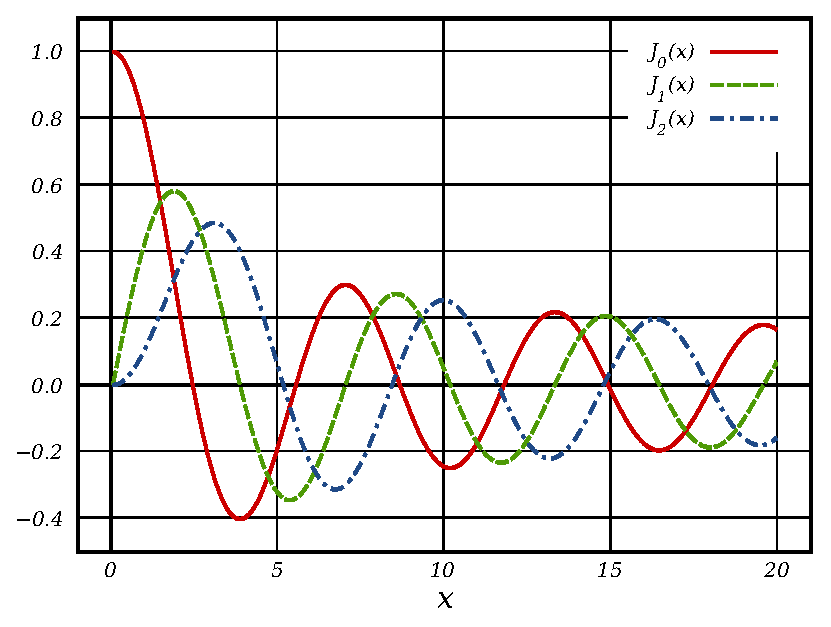
\includegraphics[width=0.5\textwidth]{besselfunctions.eps}
\caption{Bessel-functions source: $ https://de.wikipedia.org/wiki/Besselsche_Differentialgleichung$}
\label{fig:besself}
\end{center}
\end{figure}

We combine the two solutions (\eqref{eq:ansatz05} and \eqref{eq:ansatz06}) for the solution of \eqref{eq:laplcyl}:

\begin{equation}
V=Ce^{-\lambda z}J_0(\lambda r) ~~~,~~~ V=Ce^{\lambda z}J_0(\lambda r) \label{eq:ansatz07}
\end{equation}
$\lambda$ varies from $0$ to $\infty$ and $C$ varies in dependence of $\lambda$. Than we write a general solution of the potential \eqref{eq:laplcyl}:
\begin{equation}
V=\int\limits_{0}^{\infty}\left(\phi(\lambda)e^{-\lambda z}+\psi(\lambda)e^{\lambda z}\right)J_0(\lambda r) d\lambda \label{eq:sol-lapleq}
\end{equation}

Where $\phi(\lambda)$ and $\psi(\lambda)$ are arbitrary functions of $\lambda$.

\subsubsection*{Potential of homogeneous halfspace}
Starting of with the potential in cylindrical coordinates:
\begin{equation}
V=\frac{I\rho}{2\pi\sqrt{r^2+z^2}}\label{eq:2-20}
\end{equation}
Looking at the \textit{Lipschitz-Integral}:
\begin{equation}
\int\limits_{0}^{\infty}e^{-\lambda z}J_0(\lambda r)d\lambda=\frac{1}{\sqrt{r^2+z^2}} \label{eq:lipschitzint}
\end{equation}

Now using \eqref{eq:lipschitzint} we write \eqref{eq:2-20} as:
\begin{equation}
V=\frac{\rho_1 I}{2\pi}\int\limits_{0}^{\infty}e^{-\lambda z}J_0(\lambda r)d\lambda
\end{equation}

The general solution \eqref{eq:sol-lapleq} can now be written:
\begin{equation}
V=\frac{\rho_1 I}{2\pi}\int\limits_{0}^{\infty}\left(e^{-\lambda z}+\theta(\lambda)e^{-\lambda z}+X(\lambda)e^{\lambda z}\right) J_0(\lambda r)d\lambda \label{eq:sol-lapleq-2}
\end{equation}

Where $\theta(\lambda)$ and $X(\lambda)$ are arbitrary functions of $\lambda$, and $\phi(\lambda)=\frac{\rho_1 I}{2\pi}\left(1+\theta(\lambda)\right)$ and $\psi(\lambda)=\frac{\rho_1 I}{2\pi}X(\lambda)$.

The solutions of the form \eqref{eq:sol-lapleq-2} are valid in all layers but $\theta(\lambda)$ and $X(\lambda)$ can be different for each layer $i$:
\begin{equation}
V_i=\frac{\rho_1 I}{2\pi}\int\limits_{0}^{\infty}\left(e^{-\lambda z}+\theta_i(\lambda)e^{-\lambda z}+X_i(\lambda)e^{\lambda z}\right)J_0(\lambda r) d\lambda\label{eq:sol-lapleq-3}
\end{equation}

\subsubsection*{Adaption of the solution to the boundary conditions}

Assuming we are at the layer boundaries of $z=h_i$.


\begin{compactenum}[A)]
\item Potential \eqref{eq:sol-lapleq-3} is continious at each boundary plane in the subsurface:
\begin{equation}
V_i(r,h_i)=V_{i+1}(r,h_i)
\end{equation}
This equation can only be satisfied if the integrands on both sides are equal:
\begin{equation}
\theta_i(\lambda)e^{-\lambda h_i}+X_i(\lambda)e^{\lambda h_i}=\theta_{i+1}(\lambda)e^{-\lambda h_i}+X_{i+1}(\lambda)e^{\lambda h_i} \label{eq:boundary-2-23A}
\end{equation}
\item At each boundary plane $j_z$ the boundary condition must be fulfilled that:
\begin{equation}
j_z=-\frac{1}{\rho}\frac{\partial V}{\partial z}
\end{equation} 
and so
\begin{equation}
\frac{1}{\rho_i}\left(\left(1+\theta_i(\lambda)\right)e^{\lambda h_i}-X_i(\lambda)e^{\lambda h_i}\right)=\frac{1}{\rho_{i+1}}\left(\left(1+\theta_{i+1}(\lambda)\right)e^{\lambda h_i}-X_{i+1}(\lambda)e^{\lambda h_i}\right) \label{eq:boundary-2-23B}
\end{equation}
To satisfy this condition we differentiate the expression for the potential in the first layer \eqref{eq:2-20} with respect to $z$ and then substitute $z=0$:
\begin{equation}
\frac{1}{\rho_1}\frac{\partial V_1(r,0)}{\partial z}=0 ~~~,~ \textrm{for~~} r\neq 0
\end{equation}
We thus obtain the equation:
\begin{equation}
\int\limits_{0}^{\infty}\left(-1-\theta_1(\lambda)+X_1(\lambda)\right) J_0(\lambda_r)d\lambda=0
\end{equation}
\begin{equation}
\Rightarrow \theta_1(\lambda)=X_1(\lambda) \label{eq:boundary-2-23C}
\end{equation}

\item Near the current source the potential must approach to infinity
\begin{align*}
V_\infty=\frac{\rho I}{2\pi}\frac{1}{\sqrt{r^2+z^2}}
\end{align*}
which is approaching asymtotically to the potential for a layer extending to infinite height.

\item $V\rightarrow 0$ if $z\rightarrow\infty$ 
\begin{equation}
\Rightarrow X_n=0 \label{eq:boundary-2-23D}
\end{equation}
, because otherwise $e^{\lambda z}$ would drive the potential to an infinite value at an infinite depth.

\end{compactenum}

The set of equations \eqref{eq:boundary-2-23A} - \eqref{eq:boundary-2-23D} provides a system of $2n$ equation in $2n$ unknown functions $\theta(\lambda)$ and $X(\lambda)$. To obtain the solution subsitute \eqref{eq:boundary-2-23C} into \eqref{eq:boundary-2-23A} and \eqref{eq:boundary-2-23B} and subsitute \eqref{eq:boundary-2-23D} into \eqref{eq:boundary-2-23A} and \eqref{eq:boundary-2-23B}.

For brevity, we introduce the notations:
\begin{align*}
u_i=e^{\lambda h_i}, v_i=\frac{1}{u_i}, p_i=\frac{\rho_i}{\rho_{i+1}}
\end{align*}
The system of equations then become:
\begin{align*}
(u_1+v_1)\theta_1-u_2\theta_2-v_2X_2&=0\\
(v_1-u_1)\theta_1+p_1u_1\theta_2-p_1v_1X_2&=(1-p_1)u_1\\
\vdots~~~~~~~~~~~~~~~~~~~~&\vdots\\
u_{n-1}\theta_{n-1}+v_{n-1}X_{n-1}-u_{n-1}\theta_n&=0\\
-u_{n-1}\theta_{n-1}+v_{n-1}X_{n-1}+p_{n-1}u_{n-1}\theta_n-p_{n-1}v_{n-1}X_n&=(1-p_{n-1})u_{n-1}
\end{align*}
Solution of the equations by applying \textit{Cramer's rule}. For example: Solution of a two layer case (layer 1: $\rho_1, h_1$, layer 2: $\rho_2$):
\begin{align*}
\theta_1&=\frac{ku}{1-ku} && \theta_2=\frac{k(1+u)}{1-ku}\\
X_1&=\theta_1 && X_2=0
\end{align*}
with $u=e^{-2\lambda h_1}$ and the \textit{reflection coefficient of DC} $k=\frac{\rho_2-\rho_1}{\rho_2+\rho_1}$

Interesting is the potential at the surface of the earth, with $z=0$ and \eqref{eq:boundary-2-23C}:
\begin{align}
V_0=V_1(r,z)&=\frac{\rho_1 I}{2\pi}\int\limits_{0}^{\infty}\left(1+2\theta_1\right)J_0(\lambda r)d\lambda\\
&=\frac{\rho_1 I}{2\pi}\int\limits_{0}^{\infty}K(\lambda)J_0(\lambda r)d\lambda
\end{align}
where $K(\lambda)$ is the \textit{Slichter-function}.

We consider the Lipschitz-integral:
\begin{equation}
\int\limits_{0}^{\infty}e^{-\lambda z}J_0(\lambda r)d\lambda=\frac{1}{\sqrt{r^2+z^2}}\stackrel{i=0}= \int\limits_{0}^{\infty}J_0(\lambda r)d\lambda=\frac{1}{r}
\end{equation}
\eqref{eq:sol-lapleq-3} can now be written in the form:
\begin{equation}
V_0(r)=\underbrace{\frac{I}{2\pi}\left(\frac{\rho_1}{r}\right.}_{\textrm{first layer}}\left.+\int\limits_{0}^{\infty}(T(\lambda)-\rho_1)J_0(\lambda r)d\lambda\right)
\end{equation}
with $T(\lambda)=\rho_1(1+2\theta_1(\lambda))$
Example/reminder for four point measurement:
\begin{align*}
V_1=\frac{I\rho}{2\pi}\left(\frac{1}{AM}-\frac{1}{BM}\right)
\label{eq:V0}
\end{align*}

\subsubsection{Derivation of a formula for the apparent resistivity}
Take an arbitrary DC-Array (compare Fig. \ref{fig:dc01}). Then
\begin{align*}
\Delta U=\frac{I\rho}{2\pi}\left(\frac{1}{AM}-\frac{1}{AN}-\frac{1}{BM}+\frac{1}{BN}\right)
\end{align*}
\begin{align*}
\rho_a=k\frac{\Delta U}{I}
\end{align*}
where $k$ is the geometrical factor.
If we look at experimental data with an error of 1\% for the distances between the electrodes, the error in $\rho_a$ would be 2\%. But 10\% error in the lateral direction of the electrodes results only in 1\% error in $\rho_a$.

In case of the Schlumberger array ($L=AM+MN/2$ and $a=MN$, $a\ll L$) we get a voltage decrease in U:
\begin{align*}
U&=2\left(V_0(\frac{L}{2}-\frac{a}{2}\right)-V_0\left(\frac{L}{2}+\frac{a}{2}\right)\\
&\approx -2a\frac{\partial V_0}{\partial r}\bigg|_{r=L/2}
\end{align*}
and the geometrical factor in case of Schlumberger $k=\frac{\pi}{a}\left(\left(\frac{L}{2}\right)^2-\left(\frac{a}{2}\right)^2\right)$
\begin{align*}
\rho_a(L/2)=K\frac{U}{I}=\frac{2\pi}{I}\left(\frac{L}{2}\right)^2\frac{\partial V_0}{\partial r}
\end{align*}
with $\frac{d}{dx}J_0(x)=-J_1(x)$. From eq. 2.25!!!!:

\begin{equation}
\rho_a(L/2)=\rho_1+\left(\frac{L}{2}\right)^2\underbrace{\int\limits_{0}^{\infty}(T(\lambda)-\rho_1)J_1(\lambda L/2)\lambda d\lambda}_{\textrm{Stefanescu-Integral}} \label{eq:rho_a_01}
\end{equation}

The calculations of the model response $\rho_a(L/2)$ from given model parameters $(\rho_i,h_i)$ is a forward problem. 

Given:
\begin{figure}[H]
\begin{center}
\caption{Given parameters}
\label{fig:forwardgiven}
\end{center}
\end{figure}

Now two steps are neccessary:
\begin{itemize}
\item Calculation of $T(\lambda)$
\item Integration of \eqref{eq:rho_a_01} $\rightarrow$ Stefanescu-Integral
\end{itemize}

\subsubsection{Calculation of the resistivity transform $T(\lambda)$}

For a method for the determination of $T(\lambda)$ see chapter \ref{ch:2.1.2}. Then we calculate the solution of the equation system $\theta_i$ and $X_i$ and determine $T(\lambda)$ using $T(\lambda)=\rho_1(1+2\theta_1(\lambda))$. This procedure is too time consuming for a high number of layers.

Now we derive a recursion formula using the boundary conditions A to D from \ref{ch:2.1.2}. At first a new definition:

\begin{equation}
T_i(\lambda)=\rho_1\frac{1+\theta_1(\lambda)+X_i(\lambda)e^{2\lambda t_i-1}}{1+\theta_1(\lambda)-X_i(\lambda)e^{2\lambda t_i-1}}
\label{eq:Tlambda}
\end{equation}
with $i=1,2,\ddots,n$, $t_i=h_1+h_2+\ddots+h_i$ and $t_0=0$.

Because of \eqref{eq:boundary-2-23C}: $\theta_1(\lambda)=X_1(\lambda)$, we get: $T_1(\lambda)=T(\lambda)$.

Because of \eqref{eq:boundary-2-23D}: $X_n=0$, we get: $T_n(\lambda)=\rho_n$.\\

From the boundary conditions \eqref{eq:boundary-2-23A} and \eqref{eq:boundary-2-23B}:\\

\begin{compactenum}[a)]
\item $\theta_i(\lambda)e^{-\lambda t_i}+X_i(\lambda)e^{\lambda t_i}=\theta_{i+1}(\lambda)e^{-\lambda t_i}+X_{i+1}(\lambda)e^{\lambda t_i}$\\


\item $\frac{1}{\rho_i}\left(\left(1+\theta_i(\lambda)\right)e^{-\lambda t_i}-X_i(\lambda)\right)=\frac{1}{\rho_i}\left(\left(1+\theta_{i+1}(\lambda)\right)e^{-\lambda t_i}-X_{i+1}(\lambda)\right)$
\end{compactenum}

The next steps are:
\begin{itemize}
\item Add $e^{-\lambda t_i}$ on both sides of \eqref{eq:boundary-2-23A}
\item Divide each side over the corresponding side of \eqref{eq:boundary-2-23B}
\item Cancel the left part of the new equation by $X_i(\lambda)$
\end{itemize}
Then:

\begin{equation*}
\rho_i\frac{K_i(\lambda)+e^{2\lambda t_i}}{K_i(\lambda)-e^{2\lambda t_i}}=T_{i+1}(\lambda)
\end{equation*}
with $K_i(\lambda)=\frac{1+\theta_i(\lambda)}{X_i(\lambda)}$

Now the next step is to Solve the eq. \eqref{eq:Tlambda}, insert it and short translation and solving it for $T(\lambda)$:

\begin{equation}
T_i(\lambda)=\frac{T_{i+1}+\rho_i\tanh(\lambda h_i)}{1+\frac{T_{i+1}(\lambda)}{\rho_i}\tanh(\lambda h_i)}
\label{eq:Tlambda2}
\end{equation}
which is the \textit{recursion formula of PEKERIS}.

Now start with $T_n=\rho_n$, calculate step by step $T_i(\lambda)$ until $T_1(\lambda)=T(\lambda)$ $\rightarrow$ \textit{resistivity transform}

Illustration of eq. \eqref{eq:Tlambda2}:
\begin{align*}
\lambda=\frac{1}{L/2} && T_n(\lambda)=\rho_n
\end{align*}

Two extreme values:
\begin{align*}
L/2 \rightarrow 0 && L/2 \rightarrow \infty
\end{align*}

\subsubsection*{Two layer model}

\begin{figure}[H]
\begin{center}
\resizebox{0.4\textwidth}{!}
{
\begin{pspicture}(0,-0.87890625)(4.5009375,0.85890627)
\psline[linewidth=0.04cm](0.4809375,0.8389062)(4.4809375,0.8389062)
\psline[linewidth=0.04cm](0.4809375,-0.16109376)(4.4809375,-0.16109376)
\usefont{T1}{ptm}{m}{n}
\rput(1.6523438,0.34390625){$\rho_1=5\Omega m$}
\usefont{T1}{ptm}{m}{n}
\rput(1.6423438,-0.6560938){$\rho_2=10\Omega m$}
\usefont{T1}{ptm}{m}{n}
\rput(3.4423437,0.34390625){$\h_1=1 m$}
\end{pspicture} 
}

\caption{Two layer model}
\label{fig:2layermodel}
\end{center}
\end{figure}

$T_n(\lambda)=T_2(\lambda)=10\Omega m$

\begin{enumerate}
\item $L/2 \rightarrow 0$ $\Rightarrow \lambda \rightarrow \infty \Rightarrow \tanh(\infty)\rightarrow 1$
\begin{align*}
T(\lambda)=T_1(\lambda)=\frac{T_{2}+\rho_1\tanh(\lambda h_1)}{1+\frac{T_{2}(\lambda)}{\rho_1}\tanh(\lambda h_1)}=\frac{10+5}{1+10/5}=5\Omega m
\end{align*}
\item $L/2\rightarrow \infty \Rightarrow \lambda	\rightarrow 0 \Rightarrow \tanh(0)\rightarrow 0$
\begin{align*}
T_1(\lambda)=\frac{10+0}{1+0}=10\Omega m
\end{align*}
\end{enumerate}

\begin{figure}[H]
\begin{center}
\resizebox{0.5\textwidth}{!}
{
\begin{pspicture}(0,-2.4576561)(12.062813,2.4576561)
\psline[linewidth=0.04cm,arrowsize=0.05291667cm 2.0,arrowlength=1.4,arrowinset=0.4]{->}(1.7809376,-1.8407812)(9.780937,-1.8407812)
\psline[linewidth=0.04cm,arrowsize=0.05291667cm 2.0,arrowlength=1.4,arrowinset=0.4]{->}(1.7809376,-1.8407812)(1.7809376,2.2592187)
\psbezier[linewidth=0.04,linestyle=dashed,dash=0.16cm 0.16cm](1.7809376,1.1592188)(6.7809377,1.1592188)(4.6809373,-0.74078125)(8.780937,-0.74078125)
\usefont{T1}{ptm}{m}{n}
\rput(0.9323437,2.2642188){$T(1/(L/2))$}
\usefont{T1}{ptm}{m}{n}
\rput(10.542344,-2.2357812){$\lambda=(1/(L/2))$}
\usefont{T1}{ptm}{m}{n}
\rput(1.4334375,1.2642188){10}
\usefont{T1}{ptm}{m}{n}
\rput(1.3504688,-0.6357812){5}
\end{pspicture} 
}
\caption{??????}
\label{fig:lambdaTlambda}
\end{center}
\end{figure}

\subsubsection{Solution of the Stefanescu-Integral}
An analytical solution is not possible! One of the possibilities uses the linear filter method.
\paragraph{Basic Equations of the linear filter method: The fast HANKEL-transformation}

The calculation of a function $g(r)$ from $\rho(\lambda)$ by
\begin{equation}
g(r)=\int\limits_{0}^{\infty}\rho(\lambda)J_\nu(\lambda r)\lambda d\lambda
\label{eq:hankeltransform}
\end{equation}
is defined as the \textit{HANKEL-transformation}. It expresses any given function as the weighted sum of an infinite number of Bessel-functions.

The \textit{inverse Hankel-transformation}:

\begin{equation}
\rho(\lambda)=\int\limits_{0}^{\infty}g(r)rJ_\nu(\lambda r)dr
\label{eq:hankeltransforminv}
\end{equation}

Then the Stefanescu Integral has the form of a Hankel-transformation. 


The following method to calculate the integral \eqref{eq:hankeltransform} is called the fast Hankel-transform. It provides function values for $g(r)$ at discrete points.

To solve this \textit{four steps are neccessary}:
\begin{compactenum}[1)]
\item The variables are transformed into logarithmic values.
\begin{align*}
x=\ln(r/r_0) && y=-\ln(\lambda/r_0)\\
\Rightarrow r=e^x && \lambda=e^{-y}
\end{align*}
with $r_0$ the reference length. Then:
\begin{align*}
r\lambda=e^{x-y} && dr=rdx && d\lambda=-\lambda dy
\end{align*}
Insert this into eq. \eqref{eq:hankeltransform} and \eqref{eq:hankeltransforminv}:
\begin{align*}
rg(r)=-\int\limits_{-\infty}^{\infty}\rho(\lambda)\lambda J_\nu(e^{x-y})e^{x-y} dy
\end{align*}
$\lambda\rightarrow 0, y\rightarrow \infty$ and $\lambda\rightarrow \infty, y\rightarrow -\infty$.
\begin{align*}
\lambda\rho(\lambda)=\int\limits_{-\infty}^{\infty}g(r)r J_\nu(e^{x-y})e^{x-y} dx
\end{align*}
$r\rightarrow 0, x\rightarrow -\infty$ and $ r\rightarrow \infty, x\rightarrow \infty$.

From this follow the \textit{Convolution integrals}:
\begin{align}
\begin{split}
\label{eq:convintegrals}
F(y)&=\int\limits_{-\infty}^{\infty}G(x)H(x-y)dx\\
G(x)&=\int\limits_{-\infty}^{\infty}F(y)H(x-y)dy
\end{split}
\end{align}

The requirement for the fast Hankel transformation is \textit{not} only that the integral \eqref{eq:hankeltransforminv} has the form of a Hankel transformation but it can be \textit{transferred} to a \textit{convolution integral} \eqref{eq:convintegrals}.\\


\item The function $F$ is represented in the form (by using the sampling theorem):
\begin{align}
F(y)=\sum_{j=-\infty}^{\infty}F(y_j)\operatorname{sinc}\left(\pi\frac{y-y_j}{\Delta y}\right) \label{eq:2.33}
\end{align}
with $\operatorname{sinc}(z)=\frac{\sin(z)}{z}$ and $y_j=y_0+j\Delta y$ with $y_0$ arbitrary.

Sampling is the process of converting a signal into a numeric sequence. A band limited function can only be perfectly reconstructed from a countable sequence of samples, if the band limit $B$ is not greater than half of the sampling rate. This leads to a formula for the reconstruction of the original function from it's samples:
\begin{align*}
\rho_{ny}=\frac{1}{2\Delta t}
\end{align*}

\item Inserting \eqref{eq:2.33} into \eqref{eq:convintegrals} gives:
\begin{align}
G(x)=\sum_{j=-\infty}^{\infty}c_j(x)F(y_j)
\end{align}
with $c_j(x)=\int\limits_{-\infty}^{\infty}\operatorname{sinc}\left(\pi\frac{y-y_j}{\Delta y}\right)H(x-y)dy$.

The calculation of a general function is reduced to the transformation of a sinc function.\\

\item The calculation of $G(x)$ is limited to the calculation of function values at discrete points: $x_k=x_0+k\Delta x$ with $k=...,-1,0,1,...$ and $x_0$ arbitrary and $\Delta x=\Delta y$.

Inserting in the equation of $c_j(x)$:
\begin{align*}
c_j(x_k)=c_0(x_k)
\end{align*}
and so it follows:
\begin{equation}
G(x_k)=\sum_{j=-\infty}^{\infty}c_{k-j}F(y_j)\label{eq:2.35}
\end{equation}
with $c_{k-j}=c_0(x_k-j)$.

That means only the coefficients $c_k$ will be calculated from the funtion.
\begin{align}
c_0(x)=\int\limits_{-\infty}^{\infty}H(x-y)\operatorname{sinc}\left(\pi\frac{y-y_0}{\Delta y}\right) dy
\end{align}
at the points $x_k$.
The transformation is thereby reduced to the transformation of a single sinc function. Two conclusions result from the properties of the \textit{sinc response} for the application of the fast Hankel-transformation:
\begin{enumerate}
\item Only $c_k$ with values over a lower ($k_n$) and upper ($k_0$) limit are calculated:
\begin{align*}
k_n<c_k<k_0
\end{align*}
The amount of $c_k$ can be defined as a filter, so that \eqref{eq:2.35} becomes:
\begin{equation}
G(x_k)=\sum_{j=k-k_0}^{k-k_n}c_{k-j}F(y_j)
\end{equation}
\item Due to the oscillations, zero values of $c_0(x)$ result at distances of $\Delta x$ for large and small $x$ values. By subtle choice of $x_0$ it can be reached, that values $x_k$ will be close to zero points for large and small $k$ and the function values dissapear. That means the filter will be shorter.
\end{enumerate}
\end{compactenum}

\paragraph{Calculation of a filter}
There are several possibilities to calculate values of $c_0(x)$. The first paper was published by Ghosh (1971). There exists functions $F(y)$ for which the eq. \eqref{eq:convintegrals}: $G(x)=\int F(y)H(x-y)dy$ can be solved analytically and $G(x)$ can be calculated. For such cases we apply the Fourier-transformation.

\begin{align*}
\tilde{F}(k)=\frac{1}{2\pi}\int\limits_{-\infty}^{\infty}F(y)e^{-iky}dy
\end{align*}
and $\tilde{G}(k)$ analogous. Then \eqref{eq:convintegrals} has the form of a convolution integral:

\begin{align*}
G(x)&=F(y)\ast H(x-y)\\
G(k)&=F(k)\cdot H(k)
\end{align*}
Also eq. eqref eq:2.34 has the form of a convolution integral:
\begin{align*}
c_j(x)=\int\limits_{-\infty}^{\infty}\operatorname{sinc}\left(\pi\frac{y-y_j}{\Delta y}\right)H(x-y)dy && y_0=0
\end{align*}
Therefore:
\begin{align*}
\tilde{c}_0(k)=\tilde{H}(k)\frac{1}{2\pi}\int\limits_{-\infty}^{\infty}\operatorname{sinc}\left(\pi\frac{y}{\Delta y}\right)e^{-kyi}dy
\end{align*}
with 
\begin{align*}
\frac{1}{2\pi}\int\limits_{-\infty}^{\infty}\operatorname{sinc}\left(\pi\frac{y}{\Delta y}\right)e^{-kyi}dy=\begin{cases}
\frac{\Delta y}{2\pi}~~~~, for |k|<\pi/\Delta y\\
0 ~~~~, otherwise
\end{cases}
\end{align*}
follows:
\begin{align*}
\tilde{c}_0(k)=\begin{cases}
\frac{\tilde{G}(k)}{\tilde{F}(k)}\frac{\Delta y}{2\pi}~~~~, for |k|<\pi/\Delta y\\
0~~~~, otherwise
\end{cases}
\end{align*}


\paragraph{Example of a resistivity filter}
eq. 2.27
\begin{align*}
\rho_a(L/2)=\rho_1+(L/2)^2\int\limits_{0}^{\infty}(T(\lambda)-\rho_1)J_1(\lambda L/2)\lambda d\lambda\\
x=\ln(L/2), y=-\ln(\lambda)
\end{align*}
$L/2$ in m, $\lambda is 1/m$
\begin{align*}
G(x)=\int F(y) H(x-y)dy
\end{align*}
with
\begin{align*}
G(x)&=\rho_a(e^x)-\rho_1\\
F(y)&=\rho_a(e^{-y})-\rho_1\\
H(x)&=J_1(e^x)
\end{align*}
We can now calculate the resistivity filter $c_0(k)=G(k)/F(k)$ by applying the fast HT.
Filter with 3 values per decade $\rightarrow$ Ghosh, with 6 values per decade $\rightarrow$ O'Neill, with 10 $\rightarrow$ Johansen.

For all filters:
\begin{align*}
\sum_{k=k_n}^{k_0}c_k=1
\end{align*}
Using eq. 2.37:
\begin{align*}
\rho_a(e^{x_k})=\sum_{j=k-k_0}^{k_n}c_{k-j}T(e^{-y_j})
\end{align*}

\subsection{Principle of equivalence}

We can now calculate theoretical apparent resistivities for a 1D model. For example with the Schlumberger-Array:
\begin{align*}
\rho_a(x)=\sum_{k_{min}}^{k_{max}}\underbrace{T(\lambda)}_{Pekeris}\underbrace{\rho_k}_{filter coeff.}
\end{align*}

using $\rho_1=10\Omega m, h_1=1m, \rho_2=10\Omega m, h_2=5m, \rho_3=50\Omega m$ in a three layer case results in

\begin{figure}[H]
\begin{center}

\caption{Apparent resistivity in a three layer case}
\label{fig:3lcaseappres}
\end{center}
\end{figure}

\subsubsection*{Different types of $\rho_a$-curves}
\begin{figure}[H]
\begin{center}
\scalebox{1} % Change this value to rescale the drawing.
{
\begin{pspicture}(0,-1.23)(11.06,1.23)
\psline[linewidth=0.04cm,arrowsize=0.05291667cm 2.0,arrowlength=1.4,arrowinset=0.4]{->}(0.0,-1.19)(0.0,1.21)
\psline[linewidth=0.04cm,arrowsize=0.05291667cm 2.0,arrowlength=1.4,arrowinset=0.4]{->}(0.0,-1.17)(2.66,-1.17)
\psline[linewidth=0.04cm,arrowsize=0.05291667cm 2.0,arrowlength=1.4,arrowinset=0.4]{->}(2.78,-1.21)(2.78,1.19)
\psline[linewidth=0.04cm,arrowsize=0.05291667cm 2.0,arrowlength=1.4,arrowinset=0.4]{->}(2.78,-1.19)(5.44,-1.19)
\psline[linewidth=0.04cm,arrowsize=0.05291667cm 2.0,arrowlength=1.4,arrowinset=0.4]{->}(5.58,-1.21)(5.58,1.19)
\psline[linewidth=0.04cm,arrowsize=0.05291667cm 2.0,arrowlength=1.4,arrowinset=0.4]{->}(5.58,-1.19)(8.24,-1.19)
\psline[linewidth=0.04cm,arrowsize=0.05291667cm 2.0,arrowlength=1.4,arrowinset=0.4]{->}(8.38,-1.21)(8.38,1.19)
\psline[linewidth=0.04cm,arrowsize=0.05291667cm 2.0,arrowlength=1.4,arrowinset=0.4]{->}(8.38,-1.19)(11.04,-1.19)
\psbezier[linewidth=0.04](0.0,0.25)(0.68,0.27)(0.721172,-0.4784006)(1.18,-0.43)(1.638828,-0.38159943)(1.58,0.59)(2.28,0.57)
\psbezier[linewidth=0.04](2.78,0.43)(4.02,1.11)(4.76,0.83)(5.18,-0.33)
\psbezier[linewidth=0.04](5.58,-0.41)(6.5,0.11)(6.54,0.31)(8.06,0.59)
\psbezier[linewidth=0.04](8.36,0.43)(9.38,0.25)(9.66,-0.01)(10.78,-0.75)
\usefont{T1}{ptm}{m}{n}
\rput(0.843125,1.015){H}
\usefont{T1}{ptm}{m}{n}
\rput(4.0485935,1.035){K}
\usefont{T1}{ptm}{m}{n}
\rput(6.9665623,0.935){A}
\usefont{T1}{ptm}{m}{n}
\rput(9.756719,0.935){Q}
\end{pspicture} 
}
\caption{Different types of curves (in a three layer case).}
\end{center}
\end{figure}

\begin{description}
\item[K-Type:] No difference between $\rho_a$-curves of different model, if $\rho_2\cdot h_2$ is identical.
\item[H-Type:] $h_2/\rho_2$ is identical

\end{description}
\subsubsection*{Example:}
\begin{minipage}{0.45\textwidth}
\begin{center}
\textbf{Model 1}
$\rho_1=1\Omega m, h_1=1m$\\
$\rho_2=20\Omega m, h_2=1m$\\
$\rho_1=1\Omega m$\\
\end{center}
\end{minipage}
\begin{minipage}{0.45\textwidth}
\begin{center}
\textbf{Model 2}
$\rho_1=1\Omega m, h_1=1m$\\
$\rho_2=40\Omega m, h_2=0.5m$\\
$\rho_1=1\Omega m$\\
\end{center}
\end{minipage}
in both cases: $\rho_2\cdot h_2=20\cdot 1=40\cdot 0.5$.

%\begin{figure}[H]
%\begin{center}
%XXX
%\caption{$\rho_a$ in both model cases.}
%\label{fig:modelexample}
%\end{center}
%\end{figure}
Equivalent models should be calculated as the result of interpretation:

%\begin{figure}[H]
%\begin{center}
%XXX
%\caption{Inversion result of equivalent models}
%\label{fig:eqmodels}
%\end{center}
%\end{figure}

\subsection{Interpretation of resistivity data: Inversion}

\begin{figure}[H]
\begin{center}
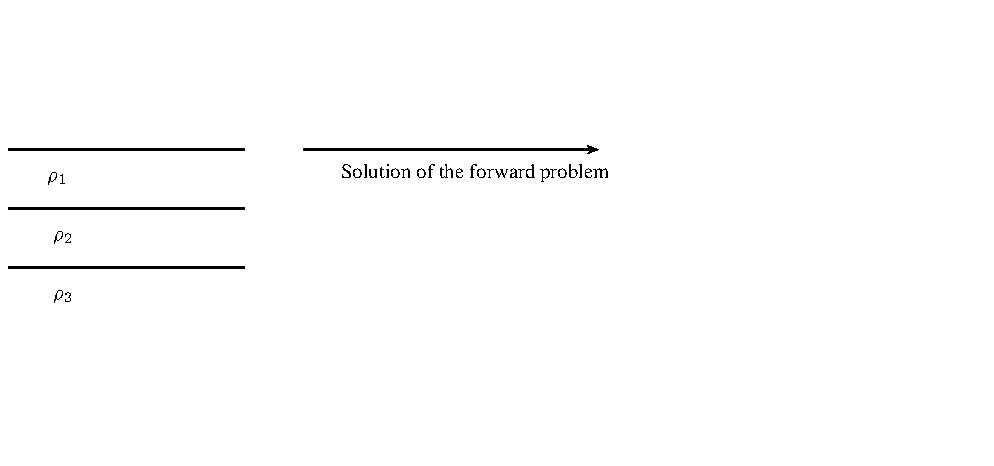
\includegraphics[width=0.7\textwidth]{invidea.eps}
\caption{Inversion idea}
\label{fig:inv01}
\end{center}
\end{figure}
The aim of the inversion is the minimization of the error function or cost function $\psi_d$ between observed and calculated apparent resistivity data. Minimize:
\begin{equation}
\psi_d=\|\vec{y}-f(\vec{m})\|^2
\end{equation}
$\vec{y}$ is the vector of measured data (e.g. $\vec{y}=(\rho_a(L/2=5m),\rho_a(L/2=10m),...)$.

$f(\vec{m}$ is the vector of calculated data.

$\psi_d$ is the norm of differences between measured and observed data.

\subsubsection{Strategies for the inversion}
Different methods to minimize the difference between measured and calculated data:
\begin{itemize}
\item Trial and error
\item method of Zohdy
\item Automatic inversion by linearisation of the forward operator $f(\vec{m})$
\end{itemize}

\paragraph{Trial and Error}

\begin{figure}[H]
\begin{center}
\resizebox{0.5\textwidth}{!}
{
\begin{pspicture}(0,-2.6034896)(7.9042706,2.6034896)
\usefont{T1}{ptm}{m}{n}
\rput(3.2217708,2.2642188){\psframebox[linewidth=0.04]{Input: Starting model $m_0$ and $y$=data}}
\usefont{T1}{ptm}{m}{n}
\rput(3.326302,0.76421875){\psframebox[linewidth=0.04]{Forward calculation $\rightarrow f(m_0)$}}
\usefont{T1}{ptm}{m}{n}
\rput(3.006302,-0.53578126){\psframebox[linewidth=0.04]{RMS small?}}
\usefont{T1}{ptm}{m}{n}
\rput(3.0766146,-2.2357812){\psframebox[linewidth=0.04]{Output: end model}}
\psline[linewidth=0.04cm,arrowsize=0.05291667cm 2.0,arrowlength=1.4,arrowinset=0.4]{->}(3.0367708,1.9592187)(3.0367708,1.0592188)
\psline[linewidth=0.04cm,arrowsize=0.05291667cm 2.0,arrowlength=1.4,arrowinset=0.4]{->}(3.0367708,0.45921874)(3.0367708,-0.24078125)
\psline[linewidth=0.04cm,arrowsize=0.05291667cm 2.0,arrowlength=1.4,arrowinset=0.4]{->}(3.0367708,-0.8407813)(3.0367708,-1.9407812)
\psline[linewidth=0.04cm](4.036771,-0.54078126)(7.1367707,-0.54078126)
\psline[linewidth=0.04cm](7.1367707,-0.54078126)(7.1367707,1.3592187)
\psline[linewidth=0.04cm,arrowsize=0.05291667cm 2.0,arrowlength=1.4,arrowinset=0.4]{->}(7.1367707,1.3592187)(3.1367707,1.3592187)
\usefont{T1}{ptm}{m}{n}
\rput(3.608802,-1.2357812){Yes}
\usefont{T1}{ptm}{m}{n}
\rput(7.6528645,0.26421875){No, new model}
\end{pspicture} 
}
\caption{Trial and error scheme}
\label{fig:trialanderror}
\end{center}
\end{figure}

with
\begin{equation}
RMS=\sqrt{\frac{1}{N}\sum_{i=1}^{N}\frac{(\rho_a^m(i)-\rho_a^c(i))^2}{(\rho_a^c(i))^2}}
\end{equation}
$\rho_a^m$ measured data, $\rho_a^c$ calculated data.

\paragraph{ZOHDY-technique}
This method is suitable for the inversion of DC-resistivity data measured by a four electrode array (Schlumberger, Wenner, ...).Utilize the principle of equivalence: The fitting of the measured data by using a resistivity model with a \textit{large} number of layers has the same quality if less layers are used.

\subsubsection*{Example:}
\begin{figure}[H]
\begin{center}
\resizebox{0.6\textwidth}{!}
{
\begin{pspicture}(0,-2.4329689)(14.081875,2.4329689)
\psline[linewidth=0.04cm,arrowsize=0.05291667cm 2.0,arrowlength=1.4,arrowinset=0.4]{->}(0.0,2.2345312)(0.0,-1.7654687)
\psline[linewidth=0.04cm,arrowsize=0.05291667cm 2.0,arrowlength=1.4,arrowinset=0.4]{->}(0.0,2.2345312)(4.0,2.2345312)
\psline[linewidth=0.04cm,arrowsize=0.05291667cm 2.0,arrowlength=1.4,arrowinset=0.4]{->}(8.0,-1.7654687)(8.0,2.2345312)
\psline[linewidth=0.04cm,arrowsize=0.05291667cm 2.0,arrowlength=1.4,arrowinset=0.4]{->}(8.0,-1.7654687)(13.1,-1.7654687)
\usefont{T1}{ptm}{m}{n}
\rput(13.611406,-2.2604687){$L/2$}
\usefont{T1}{ptm}{m}{n}
\rput(7.8214064,2.2395313){$\rho_a$}
\psline[linewidth=0.04cm](1.5,2.1345313)(1.5,1.1345313)
\psline[linewidth=0.04cm](1.5,1.1345313)(3.2,1.1345313)
\psline[linewidth=0.04cm](3.2,1.1345313)(3.2,-0.06546875)
\psline[linewidth=0.04cm](3.2,-0.06546875)(1.3,-0.06546875)
\psline[linewidth=0.04cm](1.3,-0.06546875)(1.3,-1.6654687)
\psline[linewidth=0.04cm](1.5,1.9345312)(1.7,1.9345312)
\psline[linewidth=0.04cm](1.7,1.9345312)(1.7,1.6345313)
\psline[linewidth=0.04cm](1.7,1.6345313)(1.6,1.6345313)
\psline[linewidth=0.04cm](1.6,1.6345313)(1.6,1.3345313)
\psline[linewidth=0.04cm](1.6,1.3345313)(1.9,1.3345313)
\psline[linewidth=0.04cm](1.9,1.3345313)(1.9,1.0345312)
\psline[linewidth=0.04cm](1.9,1.0345312)(2.2,1.0345312)
\psline[linewidth=0.04cm](2.2,1.0345312)(2.2,0.83453125)
\psline[linewidth=0.04cm](2.2,0.83453125)(2.5,0.83453125)
\psline[linewidth=0.04cm](2.5,0.83453125)(2.5,0.53453124)
\psline[linewidth=0.04cm](2.5,0.53453124)(2.8,0.53453124)
\psline[linewidth=0.04cm](2.8,0.53453124)(2.8,0.33453125)
\psline[linewidth=0.04cm](2.8,0.33453125)(3.3,0.33453125)
\psline[linewidth=0.04cm](3.3,0.33453125)(3.3,0.23453125)
\psline[linewidth=0.04cm](3.3,0.23453125)(2.9,0.23453125)
\psline[linewidth=0.04cm](2.9,0.23453125)(2.9,0.03453125)
\psline[linewidth=0.04cm](2.9,0.03453125)(2.5,0.03453125)
\psbezier[linewidth=0.106000006,linestyle=dotted,dotsep=0.16cm](8.0,-0.45008412)(8.0,-1.0654688)(9.5,1.9345312)(13.0,-0.06546875)
\psbezier[linewidth=0.106000006](8.1,-0.35008413)(8.1,-0.96546876)(9.1,2.0345314)(12.6,0.03453125)
\end{pspicture} 
}
\caption{Example layers in inversion}
\label{fig:inv02}
\end{center}
\end{figure}
\subsubsection*{Procedure}
\begin{compactenum}[1)]
\item Starting model with $m$ layers, where $m$ is the number of measured data. $\rho_i=\rho_{a_i}$, $t_i=(L/2)_i$. Thickness of the $i$'th layer: $h_i=(L/2)_{i+1}-(L/2)_{i}$.
Then do the forward and RMS calculation. For example RMS is 62\%.

\item Reduction of the thickness of each layer as 0.9 and then do forward and RMS calculation. Repetition of the procedure until no improvement of RMS is possible.
For example: 10 iterations reduce RMS to 12\%.

\item Determination of resistivity of each layer:
\begin{align*}
\rho_{i+1}(j)=\rho_i(j)\frac{\rho_{a_{i,obs}}(j)}{\rho_{a_{i,c}}(j)}
\end{align*}
with $i$ the number of iterations and $j$ the number of layer = $L/2$ number. $\rho_i(j)$: resistivity of the $j$'th layer of the $i$'th iteration. $\rho_{a_{i,c}}$: calculated apparent resistivity data for the $j$'th layer and $i$'th iteration.

Now do the forward calculation and calculate the RMS. Similar to step 2) repetition of the procedure (example 12\% to 1\%).
\end{compactenum}
\subsubsection*{Disadvantage:}
No good result, if data points have relatively large noise, because every data point is a layer.

\paragraph{Inversion by linearization of the forward operator}
The aim of the inversion is to minimize the cost function $\psi_d$. A measure for the error:
\begin{equation}
X^2=\frac{1}{N}\sum_{i=1}^{N}\frac{(y_i-f_i)^2}{\sigma_i^2}
\end{equation}
where $n$ is the number of measured data and calculated data. $\sigma$ is the standard deviation. 
\textit{Mathematically:} $\min \|y-f(m)\|^2$ (To solve use e.g. Gauss Newton method). The problem is not linear, therefore linearise $f(m)$ or $\psi_d$.

The linearisation can be done by a Taylor expansion of the forward operator $f(m)$ for small model changes $\Delta m$ close to the starting model $m_0$:
\begin{align}
f(m_0+\delta m)=f(m_0)+\frac{\partial f(m_0)}{\partial m_0}\Delta m\approx f(m_0)+\tens{J}\Delta m
\end{align}
where $\tens{J}$ is the jacobian or sensitivity matrix. It describes the influence of model parameters on the model response. eq. 2.38 can now be written as:
\begin{equation}
\psi_d(m_a)=\|y-f(m_0)\|^2=(y-f(m_0))^T(y-f(m_0))
\end{equation}
using the Taylor expansion:
\begin{equation}
\psi_d(m_0+\Delta m)=\|y-f(m_0+\Delta m)\|^2=(y-f(m_0+\Delta m))^T(y-f(m_0+\Delta m))
\end{equation}
Set eq. 2.40 in eq. 2.42
\begin{equation}
\psi_d(m_0+\Delta m)=\|y-f(m_0)-\tens{J}\Delta m\|^2=(y-f(m_0)-\tens{J}\Delta m)^T(y-f(m_0)-\tens{J}\Delta m)
\end{equation}
Calculation of the extreme of $\psi_d$:
\begin{align*}
\frac{\partial \psi_d(m_0+\Delta m)}{\partial \Delta m}=0=\frac{\partial }{\partial \Delta m}(y-f(m_0)-\tens{J}\Delta m)^T(y-f(m_0)-\tens{J}\Delta m)
\end{align*}
with $\Delta d=y-f(m_0)$:
\begin{align*}
0&=\frac{\partial }{\partial \Delta m}(\Delta d-\tens{J}\Delta m)^T(\Delta d-\tens{J}\Delta m)\\
&=\frac{\partial }{\partial \Delta m}(\Delta d^T\Delta d-\Delta d^T\tens{J}\Delta m-\Delta m J^T\Delta d +\Delta m^TJ^TJ\Delta m)\\
&=2J^T\Delta d-2J^TJ\Delta m\\
\Leftrightarrow J^TJ\Delta m&=J^T\Delta d
\end{align*}
Normal equation: Solution for this equation according to $\Delta m$
\begin{equation}
\Delta m=(J^TJ)^{-1}J^T\Delta d\label{eq:solutioninv}
\end{equation}
For the linear case the minima of $\psi_d$ can be reached after one iteration. For the non-linear case $m_1=m_0+\Delta m$, $m_2=m_1+\Delta m$, so the solution will be iteratively improved!


\textit{Problem:} No solution of \eqref{eq:solutioninv} if $(J^T J)$ is singular, or in other words $\det(J^TJ)=0$. To stabilize it
\begin{align*}
\Delta m(J^TJ+\beta I)^{-1}J^T\Delta d
\end{align*}
with $\beta$ the damping factor and $I$ the identity matrix. The solution according to the eq. is known as \textit{Marquardt-Levenberg method}.

\subsection{Solution of the 2D DC forward problem}
\begin{figure}[H]
\begin{center}
\resizebox{0.6\textwidth}{!}
{
\begin{pspicture}(0,-1.5789063)(12.715625,1.5589062)
\psline[linewidth=0.04cm](0.0,0.5389063)(9.0,0.5389063)
\psline[linewidth=0.04cm](3.0,0.5389063)(3.0,-0.86109376)
\psline[linewidth=0.04cm](3.0,-0.86109376)(5.0,-0.86109376)
\psline[linewidth=0.04cm](5.0,-0.86109376)(5.0,0.5389063)
\psline[linewidth=0.04cm,linestyle=dashed,dash=0.16cm 0.16cm](3.0,0.5389063)(5.0,1.5389062)
\psline[linewidth=0.04cm,linestyle=dashed,dash=0.16cm 0.16cm](5.0,0.5389063)(7.0,1.5389062)
\usefont{T1}{ptm}{m}{n}
\rput(3.9014063,-0.15609375){$\sigma_2$}
\usefont{T1}{ptm}{m}{n}
\rput(1.9014063,-1.3560938){$\sigma_1$}
\psline[linewidth=0.04cm,arrowsize=0.05291667cm 2.0,arrowlength=1.4,arrowinset=0.4]{->}(11.0,0.5389063)(11.0,-0.86109376)
\psline[linewidth=0.04cm,arrowsize=0.05291667cm 2.0,arrowlength=1.4,arrowinset=0.4]{->}(11.0,0.5389063)(12.4,0.5389063)
\psline[linewidth=0.04cm,arrowsize=0.05291667cm 2.0,arrowlength=1.4,arrowinset=0.4]{->}(11.0,0.5389063)(12.0,1.2389063)
\usefont{T1}{ptm}{m}{n}
\rput(12.585468,0.44390625){x}
\usefont{T1}{ptm}{m}{n}
\rput(12.287812,1.3439063){y}
\usefont{T1}{ptm}{m}{n}
\rput(11.2734375,-0.9560937){z}
\end{pspicture} 
}

\caption{asdfasdf}
\label{fig:solution2DDC}
\end{center}
\end{figure}

\subsubsection*{Basic equations:}
Ohm's law:
\begin{align*}
j=\sigma E\\
E=-\nabla V\\
j=-\sigma \nabla V
\end{align*}
By using the charge retention over a volume, the continuity equation can now be written as:
\begin{equation}
\nabla j=\frac{\partial q}{\partial t}\delta(x)\delta(y)\delta(z)\label{eq:poisson02}
\end{equation}
The charge density $q$ is represented at a point in the cartesian coordinates $(x,y,z)$ with the Dirac-distribution $\delta(x)$.

\begin{align}
-\nabla\left(\sigma(x,y,z)\nabla V(x,y,z)\right)=\frac{\partial q}{\partial t}\delta(x_s)\delta(y_s)\delta(z_s)
\end{align}
The \textit{Poisson equation}, with $x_s,y_s,z_s$ the coordinates of the source point. By using the vector equation $\nabla\cdot (\phi A) = \nabla\phi A +\phi\nabla \cdot A)$ with $A=\nabla V$ and $\phi=\sigma$. Then the equation \eqref{eq:poisson02} will be:
\begin{equation}
\nabla\sigma(x,y,z)\nabla V(x,y,z)+\sigma(x,y,z)\nabla^2 V(x,y,z)=-\frac{\partial q}{\partial t}\delta(x_s)\delta(y_s)\delta(z_s)\label{eq:poisson03}
\end{equation}
No change of electrical conductivity in y-direction so we have a 2D problem. $\Rightarrow \frac{\partial}{\partial y}\sigma(x,y,z)=0$.

Application of this condition to \eqref{eq:poisson02} and \eqref{eq:poisson03}:
\begin{align}
-\nabla\cdot(\sigma\nabla V)&=\frac{\partial q}{\partial t}\delta(x_s)\delta(y_s)\delta(z_s)\\
\nabla\sigma\cdot\nabla V+\sigma\nabla^2 V&=-\frac{\partial q}{\partial t}\delta(x_s)\delta(y_s)\delta(z_s)
\end{align}
Using the vector equation: $\nabla A\cdot\nabla B=\frac{1}{2}(-A\nabla^2 B + \nabla^2(AB)-B\nabla^2 A)$ with $A=\sigma$ and $B=V$ we get:

\begin{align*}
\nabla^2(\sigma(x,z)V(x,y,z))+\sigma(x,z)\nabla^2 V(x,y,z)-V(x,y,z)\nabla^2\sigma(x,z)=-2\frac{\partial q}{\partial t}\delta(x_s)\delta(y_s)\delta(z_s)
\end{align*}
Spatial distribution of the potential $V \rightarrow$ 3D, spatial distribution of the conductivity $\sigma \rightarrow$ 2D. Therefore the solution in this form is not possible.

The $y$-dependence of the potential can now be eliminated by the \textit{Fourier-cosine transformation}:
\begin{align*}
\tilde{V}(x,K_y,z)=\int\limits_{0}^{\infty}V(x,y,z)\cos(K_y y)dy
\end{align*}
3D $V(x,y,z)$ is due to point source at $(x_s,y_s,z_s)$ over a 2D conductivity structure is reduced to a 2D transformed potential $\tilde{V}(x,K_y,z)$, with $K_y$ the wave number.

For $\tilde{V}(x,K_y,z)$ the solution

\begin{align}
\nabla^2(\sigma(x,z)\tilde{V}(x,K_y,z))+\sigma(x,z)\nabla^2 \tilde{V}(x,K_y,z)-\tilde{V}(x,K_y,z)\nabla^2\sigma(x,z)-2K_y\sigma(x,z)\tilde{V}(x,K_y,z)=-2Q\delta(x_s)\delta(z_s)\label{eq:vtildeeq}
\end{align}
is looked for with $Q\delta(x_s)\delta(z_s)=\frac{1}{2}\frac{\partial q}{\partial t}$

The relationship between the stationary current density $Q$ and the current:

\begin{align*}
Q=\frac{I}{2\Delta A}
\end{align*}
where $\Delta A$ is the area around the current electrodes.

The eq. \eqref{eq:vtildeeq} is solved for different wave numbers. Afterwards do the inverse transformation:

\begin{equation*}
V(x,y,z)=\frac{2}{\pi}\int\limits_{0}^{\infty}\tilde{V}(x,K_y,z)\cos(K_y y)dK_y
\end{equation*}
Numerical solution of \eqref{eq:vtildeeq} with \textit{boundary conditions} (2D forward modelling). The boundary conditions are:

\begin{compactenum}[a)]
\item $V(x,y,z)$ is continuous between two media with different conductivity $\sigma$.
\item $V(x,y,z)\rightarrow 0$ if $z\rightarrow\infty$
\item $j_n$ is also continuous
\end{compactenum}

Now discretization of the subsurface and solution of \eqref{eq:vtildeeq} with (for example) finite differences:

\begin{figure}[H]
\begin{center}
\resizebox{0.4\textwidth}{!}
{
\begin{pspicture}(0,-2.7417188)(5.414375,2.7617188)
\psline[linewidth=0.04cm](0.394375,2.2782812)(0.394375,-2.7217188)
\psline[linewidth=0.04cm](1.394375,2.2782812)(1.394375,-2.7217188)
\psline[linewidth=0.04cm](2.394375,2.2782812)(2.394375,-2.7217188)
\psline[linewidth=0.04cm](3.394375,2.2782812)(3.394375,-2.7217188)
\psline[linewidth=0.04cm](4.394375,2.2782812)(4.394375,-2.7217188)
\psline[linewidth=0.04cm](0.394375,2.2782812)(5.394375,2.2782812)
\psline[linewidth=0.04cm](0.394375,1.2782812)(5.394375,1.2782812)
\psline[linewidth=0.04cm](0.394375,0.27828124)(5.394375,0.27828124)
\psline[linewidth=0.04cm](0.394375,-0.7217187)(5.394375,-0.7217187)
\psline[linewidth=0.04cm](0.394375,-1.7217188)(5.394375,-1.7217188)
\usefont{T1}{ptm}{m}{n}
\rput(0.24125,2.4832811){1}
\usefont{T1}{ptm}{m}{n}
\rput(1.3729688,2.5832813){2}
\usefont{T1}{ptm}{m}{n}
\rput(2.3620312,2.5832813){3}
\usefont{T1}{ptm}{m}{n}
\rput(3.3753126,2.5832813){4}
\usefont{T1}{ptm}{m}{n}
\rput(0.07296875,1.2832812){2}
\usefont{T1}{ptm}{m}{n}
\rput(0.06203125,0.28328124){3}
\usefont{T1}{ptm}{m}{n}
\rput(0.0753125,-0.71671873){4}
\psline[linewidth=0.04cm,arrowsize=0.05291667cm 2.0,arrowlength=1.4,arrowinset=0.4]{->}(6.494375,-0.42171875)(3.994375,-0.32171875)
\usefont{T1}{ptm}{m}{n}
\rput(7.795781,-0.41671875){$\sigma = const$}
\end{pspicture} 
}
\caption{Finite differences grid}
\label{fig:fdgrid}
\end{center}
\end{figure}
Calculation of the potential at the knots of the mesh and afterwards $\rho_a=K\frac{\Delta V}{I}$


\section*{Electromagnetic methods}
\section{Electromagnetic induction}
\subsection{Principle of EM-induction as an example of transformer}
The simplifications are 1 winding, no $\mu_r$ core.

\begin{figure}[H]
\begin{center}
\resizebox{0.4\textwidth}{!}
{
\begin{pspicture}(0,-2.3329687)(5.8628125,2.3329687)
\psline[linewidth=0.04cm](4.5809374,0.03453125)(3.5809374,0.03453125)
\psbezier[linewidth=0.04](3.5809374,0.03453125)(3.5809374,-0.7654688)(1.9361359,-1.6209651)(1.1809375,-0.96546876)(0.42573914,-0.3099724)(0.98633593,1.2876666)(1.8809375,1.7345313)(2.7755392,2.181396)(3.0244977,1.8654193)(3.5809374,1.0345312)
\psline[linewidth=0.04cm](3.5809374,1.0345312)(4.5809374,1.0345312)
\psline[linewidth=0.04cm](4.5809374,1.0345312)(4.5809374,0.63453126)
\psline[linewidth=0.04cm](4.5809374,0.33453125)(4.5809374,0.03453125)
\usefont{T1}{ptm}{m}{n}
\rput(5.342344,0.53953123){$V_p$}
\psline[linewidth=0.04cm,arrowsize=0.05291667cm 2.0,arrowlength=1.4,arrowinset=0.4]{->}(1.9809375,-1.3654687)(1.9809375,-1.9654688)
\usefont{T1}{ptm}{m}{n}
\rput(2.1423438,-2.1604688){$F$}
\psline[linewidth=0.04cm,arrowsize=0.05291667cm 2.0,arrowlength=1.4,arrowinset=0.4]{->}(0.6809375,0.43453124)(1.0809375,1.2345313)
\psline[linewidth=0.04cm,arrowsize=0.05291667cm 2.0,arrowlength=1.4,arrowinset=0.4]{->}(3.4809375,1.5345312)(2.8809376,2.0345314)
\usefont{T1}{ptm}{m}{n}
\rput(3.8423438,2.1395311){$V_p$}
\usefont{T1}{ptm}{m}{n}
\rput(0.76234376,1.1395313){$U_{ind}$}
\end{pspicture} 
}
\caption{EM Spule}
\label{fig:em01}
\end{center}
\end{figure}
\subsubsection*{Primary coil}
Alternating current voltage: $V_p=V_{p_0}\sin(\omega t)$ produces magnetic field flux $F$, $F$ produces induced voltage $U_{ind}=-V_p=\frac{dF}{dt}$ (Lentz law). The induced voltage is orientated in the opposite direction of $\frac{dF}{dt}$.
\begin{align*}
F=\int V_p dt=-V_{p_0}\cos(1/\omega)\\
V_p\sin(\omega t)=\frac{dF}{dt}=AL\dot{I}\\
\Rightarrow I=-I_0\cos(\omega t)
\end{align*}

\subsubsection*{Secondary coil}
\begin{figure}[H]
\begin{center}
\resizebox{0.4\textwidth}{!}
{
\begin{pspicture}(0,-1.9211804)(5.8228126,1.9211805)
\psline[linewidth=0.04cm](4.5809374,-0.24568419)(3.5809374,-0.24568419)
\psbezier[linewidth=0.04](3.5809374,-0.24568419)(3.5809374,-1.0456842)(1.9361359,-1.9011805)(1.1809375,-1.2456841)(0.42573914,-0.59018785)(0.98633593,1.007451)(1.8809375,1.4543158)(2.7755392,1.9011805)(3.0244977,1.5852038)(3.5809374,0.7543158)
\psline[linewidth=0.04cm](3.5809374,0.7543158)(4.5809374,0.7543158)
\psline[linewidth=0.04cm](4.5809374,0.7543158)(4.5809374,0.35431582)
\psline[linewidth=0.04cm](4.5809374,0.054315805)(4.5809374,-0.24568419)
\usefont{T1}{ptm}{m}{n}
\rput(5.322344,0.25931582){$R_s$}
\psline[linewidth=0.04cm,arrowsize=0.05291667cm 2.0,arrowlength=1.4,arrowinset=0.4]{->}(0.6809375,0.1543158)(1.0809375,0.9543158)
\usefont{T1}{ptm}{m}{n}
\rput(0.6123437,0.8593158){$U_{s}$}
\psframe[linewidth=0.04,dimen=outer](4.7809377,0.35431582)(4.3809376,0.054315805)
\end{pspicture} 
}
\caption{Secondary coil}
\label{fig:em02}
\end{center}
\end{figure}
$F$ produces secondary induced voltage:
\begin{align*}
U_s=-\frac{dF}{dt}=-V_{p_0}\sin(\omega t)
\end{align*}
Current drain due to Ohmic resistance
\begin{align*}
I_s=\frac{U_s}{R_s}=-V_{p_0}\sin(\omega t)/R_s
\end{align*}
$I_s$ produces additional magnetic flux:
\begin{align*}
F_s=\mu_0HA=\mu_0\frac{I}{l}A=-\mu_0\frac{r}{2}V_{p_0}\sin(\omega t)/R_s
\end{align*}
which generates an additional voltage:
\begin{align*}
V_{p_s}=-\frac{dF}{dt}=(\omega)\frac{r}{2}V_{p_0}\cos(\omega t)/R_s
\end{align*}

\subsection{Induction in the conductive subsurface}

Primary current $\rightarrow$ current system in the ionosphere or artificial sources.

Secondary coil $\rightarrow$ conductive subsurface

\subsubsection*{Geomagnetic Depth Sounding}
Aim: Derivation of in-situ conductivity from the observation of time varying electromagnetic fields at the earth surface.

\begin{figure}
\begin{center}
\resizebox{0.5\textwidth}{!}
{
\begin{pspicture}(0,-3.79)(7.0009375,3.75)
\psline[linewidth=0.04cm](0.9809375,1.75)(6.9809375,1.75)
\psline[linewidth=0.04cm](0.9809375,-1.25)(6.9809375,-1.25)
\psellipse[linewidth=0.04,dimen=outer](3.9809375,2.9)(2.0,0.85)
\psellipse[linewidth=0.04,linestyle=dashed,dash=0.16cm 0.16cm,dimen=outer](4.0309377,-3.0)(2.05,0.75)
\psline[linewidth=0.08cm,linestyle=dashed,dash=0.16cm 0.16cm,arrowsize=0.05291667cm 2.0,arrowlength=1.4,arrowinset=0.4]{->}(4.0809374,-3.75)(3.8809376,-3.75)
\psline[linewidth=0.08cm,linestyle=dashed,dash=0.16cm 0.16cm,arrowsize=0.05291667cm 2.0,arrowlength=1.4,arrowinset=0.4]{->}(3.9809375,2.05)(4.1809373,2.05)
\psline[linewidth=0.04cm,arrowsize=0.05291667cm 2.0,arrowlength=1.4,arrowinset=0.4]{->}(3.9809375,-1.25)(3.2809374,-0.55)
\psline[linewidth=0.04cm,arrowsize=0.05291667cm 2.0,arrowlength=1.4,arrowinset=0.4]{->}(3.9809375,-1.25)(3.2809374,-1.85)
\usefont{T1}{ptm}{m}{n}
\rput(3.8923438,-1.845){$B_i$}
\usefont{T1}{ptm}{m}{n}
\rput(3.9223437,-0.545){$B_e$}
\usefont{T1}{ptm}{m}{n}
\rput(0.41234374,-1.245){$z=0$}
\end{pspicture} 
}
\caption{Geomagnetic sounding}
\label{fig:em03}
\end{center}
\end{figure}

Primary source region: Ionosphere, magnetosphere, where primary currents are flowing. Secondary source region: Conductive earth layers where secondary currents are flowing.

We observe at the earth surface: 
\begin{compactenum}[a)]
\item Geomagnetic time variations $B(t)$ consisting of external $B^e$ and of interior $B^I$ part.

\textit{Tendency}: In the horizontal components constructive interaction. Destructive interaction for the vertical component.

\item Telluric $E(t)$ variations for induced currents in the subsurface

\textit{Tendency}: Strong telluric currents at near surface conductivity contrasts.
\end{compactenum}

\subsection{Basic Elements}
\subsubsection{Notation and units}
\begin{description}
\item[1. Position vector:] In spherical coordinates $(r,\theta,\lambda)$ with $r$ the distance from the Earth center, $\theta$ the polar distance and $\lambda$ the length or longitude.

In plane coordinates: $z$ is the depth, $x$ the North direction and $y$ the East direction.

\item[2. Physical base items:]~\\
$\vec{B}$: magnetic induction in nT $=10^{-9}$ Vsm$^{-2}$. 

$\vec{E}$: electric field in mV/km $=10^{-6}$ V/m.

$\vec{j}$: electric current density in A/m$^2$.

$\eta$: electric charge density in As/m$^3$.


\item[3. Material constants:] ~\\
$\epsilon,\mu$: electric permittivity and magnetic permittivity

$\mu_0=4\pi\cdot 10^{-7}$ Vs/Am

$\epsilon_0=8.85\cdot 10^{-12}$ As/Vm

$\sigma$: conductivity in S/m

$\rho$: resistivity in $\Omega$ m

\item[4. Material equations:]~\\

$\vec{D}=\epsilon\epsilon_0\vec{E}$: electrical displacement

$\vec{B}=\mu\mu_0\vec{H}$: $\vec{H}$ the magnetic field strength

????????

\item[5. Ranges:]~\\

Global Earth magnetic field: $3-6\cdot 10^4$ nT 

Earth magnetic variations: 1-100 nT

Telluric variations: 0.1 - 10 mV/km

Earth electric soil potential: 10 mV
\end{description}

$\mu=1+K$ with $K<10^{-2}$ for rocks. Therefore $\mu=1$ for the following derivations. $\epsilon= 1-80$ (water).

\begin{tabularx}{\textwidth}{c|c|c|c}
No. & Conductivity of & Charge carrier & T-dependce\\
\hline
1 & Gases & Ions, dust particles aerosols & - \\
2 & Semi conductors & electrons & with $T$ increasing according to $e^{-A/k_B T}$, $A$: activation energy\\
3 & Electrolyt & Ions & $p$ dependence of concentration of ions\\
4 & Metal & free electrons & Drecreasing with increasing $T$
\end{tabularx}

\begin{compactenum}[1)]
\item Atmosphere: $\rho\sim 10^{15}\Omega$m
\item Crystal: $\rho\sim 10^{7}\Omega$m
\item Sea water: $\rho\sim 0.25\Omega$m
\item Earth's core: $\rho\sim 10^{-5}\Omega$m
\end{compactenum}


\begin{figure}[H]
\begin{center}
\resizebox{0.6\textwidth}{!}
{
\begin{pspicture}(0,-4.2992187)(15.759687,4.3192186)
\psline[linewidth=0.04cm](0.9578125,3.1207812)(12.957812,3.1207812)
\psline[linewidth=0.04cm,arrowsize=0.05291667cm 2.0,arrowlength=1.4,arrowinset=0.4]{->}(0.9578125,3.4207811)(0.9578125,-4.079219)
\psline[linewidth=0.04cm](1.9578125,3.4207811)(1.9578125,3.1207812)
\psline[linewidth=0.04cm](2.9578125,3.4207811)(2.9578125,3.1207812)
\psline[linewidth=0.04cm](3.9578125,3.4207811)(3.9578125,3.1207812)
\psline[linewidth=0.04cm](4.9578123,3.4207811)(4.9578123,3.1207812)
\psline[linewidth=0.04cm](5.9578123,3.4207811)(5.9578123,3.1207812)
\psline[linewidth=0.04cm](6.9578123,3.4207811)(6.9578123,3.1207812)
\psline[linewidth=0.04cm](7.9578123,3.4207811)(7.9578123,3.1207812)
\psline[linewidth=0.04cm](8.957812,3.4207811)(8.957812,3.1207812)
\psline[linewidth=0.04cm](9.957812,3.4207811)(9.957812,3.1207812)
\psline[linewidth=0.04cm](10.957812,3.4207811)(10.957812,3.1207812)
\psline[linewidth=0.04cm](11.957812,3.4207811)(11.957812,3.1207812)
\psline[linewidth=0.04cm](12.957812,3.4207811)(12.957812,3.1207812)
\psline[linewidth=0.04cm](0.7578125,1.1207813)(0.9578125,1.1207813)
\psline[linewidth=0.04cm](0.7578125,-0.87921876)(0.9578125,-0.87921876)
\psline[linewidth=0.04cm](0.7578125,-2.8792188)(0.9578125,-2.8792188)
\usefont{T1}{ptm}{m}{n}
\rput(0.98859376,3.8257813){-5}
\usefont{T1}{ptm}{m}{n}
\rput(2.9854689,3.8257813){-3}
\usefont{T1}{ptm}{m}{n}
\rput(4.9784374,3.8257813){-1}
\usefont{T1}{ptm}{m}{n}
\rput(5.9348435,3.8257813){0}
\usefont{T1}{ptm}{m}{n}
\rput(7.936406,3.8257813){2}
\usefont{T1}{ptm}{m}{n}
\rput(9.93875,3.8257813){4}
\psframe[linewidth=0.04,dimen=outer](5.7578125,2.9207811)(4.9578123,2.6207812)
\psframe[linewidth=0.04,dimen=outer](7.8578124,2.9207811)(5.9578123,2.6207812)
\psframe[linewidth=0.04,dimen=outer](9.857813,2.9207811)(8.057813,2.6207812)
\psline[linewidth=0.04cm](9.957812,2.8207812)(9.957812,1.7207812)
\psline[linewidth=0.04cm](9.957812,1.7207812)(10.957812,1.7207812)
\psline[linewidth=0.04cm](10.957812,1.7207812)(10.957812,2.8207812)
\psbezier[linewidth=0.04](9.957812,1.7207812)(7.7578125,1.4207813)(6.2908163,0.5202365)(6.2578125,-0.17921875)(6.2248087,-0.878674)(7.2578125,-0.37921876)(7.7578125,-1.0792187)(8.2578125,-1.7792188)(6.563985,-1.3792378)(6.5578127,-1.7792188)(6.55164,-2.1791997)(7.1578126,-1.9792187)(7.1578126,-2.3792188)(7.1578126,-2.7792187)(4.2578125,-3.8792188)(1.4578125,-4.2792187)
\usefont{T1}{ptm}{m}{n}
\rput(14.379219,4.125781){$\rho(\Omega m)$}
\psline[linewidth=0.04cm,arrowsize=0.05291667cm 2.0,arrowlength=1.4,arrowinset=0.4]{->}(12.857813,2.2207813)(11.157812,2.2207813)
\usefont{T1}{ptm}{m}{n}
\rput(14.177969,2.2257812){upper earth crust}
\usefont{T1}{ptm}{m}{n}
\rput(0.43671876,-3.8742187){z (km)}
\usefont{T1}{ptm}{m}{n}
\rput(0.2903125,-2.8742187){1000}
\usefont{T1}{ptm}{m}{n}
\rput(0.4003125,-0.87421876){100}
\usefont{T1}{ptm}{m}{n}
\rput(0.4103125,1.1257813){10}
\usefont{T1}{ptm}{m}{n}
\rput(5.410625,2.4257812){Ocean}
\usefont{T1}{ptm}{m}{n}
\rput(7.0803127,2.4257812){Sediments}
\usefont{T1}{ptm}{m}{n}
\rput(8.906094,2.4257812){Crystalline}
\end{pspicture} 
}
\caption{Resistivity structure on Earth with depth}
\label{fig:resdepth}
\end{center}
\end{figure}
The upper earth crust has conductive anomalies in different regions.

\begin{figure}
\begin{center}
\resizebox{0.5\textwidth}{!}
{
\begin{pspicture}(0,-3.5534375)(11.012813,3.5534375)
\psline[linewidth=0.04cm,arrowsize=0.05291667cm 2.0,arrowlength=1.4,arrowinset=0.4]{->}(0.9928125,2.5634375)(0.9928125,-3.4365625)
\psline[linewidth=0.04cm,arrowsize=0.05291667cm 2.0,arrowlength=1.4,arrowinset=0.4]{->}(0.9928125,2.5634375)(10.992812,2.5634375)
\psline[linewidth=0.04cm,linestyle=dashed,dash=0.16cm 0.16cm,arrowsize=0.05291667cm 2.0,arrowlength=1.4,arrowinset=0.4]{->}(2.9928124,2.5634375)(2.9928124,1.5634375)
\psline[linewidth=0.04cm,linestyle=dashed,dash=0.16cm 0.16cm,arrowsize=0.05291667cm 2.0,arrowlength=1.4,arrowinset=0.4]{->}(4.9928126,2.5634375)(4.9928126,0.5634375)
\psline[linewidth=0.04cm,linestyle=dashed,dash=0.16cm 0.16cm,arrowsize=0.05291667cm 2.0,arrowlength=1.4,arrowinset=0.4]{->}(6.9928126,2.5634375)(6.9928126,-0.9365625)
\psline[linewidth=0.04cm,linestyle=dashed,dash=0.16cm 0.16cm,arrowsize=0.05291667cm 2.0,arrowlength=1.4,arrowinset=0.4]{->}(8.992812,2.5634375)(8.992812,-3.2365625)
\usefont{T1}{ptm}{m}{n}
\rput(2.9223437,2.9684374){Pulsation (1 min)}
\usefont{T1}{ptm}{m}{n}
\rput(4.95375,3.3684375){Variations (1h)}
\usefont{T1}{ptm}{m}{n}
\rput(7.0021877,2.8684375){Diurnal variations (1d)}
\usefont{T1}{ptm}{m}{n}
\rput(9.022187,3.2684374){Dst variations (4d)}
\usefont{T1}{ptm}{m}{n}
\rput(0.46171874,-3.3315625){z (km)}
\psline[linewidth=0.04cm](0.7928125,-2.4365625)(0.9928125,-2.4365625)
\psline[linewidth=0.04cm](0.7928125,-0.4365625)(0.9928125,-0.4365625)
\psline[linewidth=0.04cm](0.7928125,1.5634375)(0.9928125,1.5634375)
\usefont{T1}{ptm}{m}{n}
\rput(0.5453125,1.5684375){10}
\usefont{T1}{ptm}{m}{n}
\rput(0.4353125,-0.4315625){100}
\usefont{T1}{ptm}{m}{n}
\rput(0.3253125,-2.4315624){1000}
\end{pspicture} 
}
\caption{Variations}
\label{fig:em04}
\end{center}
\end{figure}


HERE LECTURE FROM 30.11.2015!!!!

%
%\subsubsection*{Solution for the homogeneous halfspace}
%
%1) Solution for TE-source fields $\rightarrow E_z=0$:
%
%Eq. 3.13. $z>0$
%
%\begin{align*}
%\hat{E}_x=A_xe^{-kz}+B_xe^{kz}\\
%\hat{E}_y=A_ye^{-kz}+B_ye^{kz}\\
%\hat{B}_x=\frac{1}{i\omega}\frac{d\hat{E}_y}{dz}\\
%\hat{B}_y=\frac{1}{i\omega}\frac{d\hat{E}_x}{dz}\\
%\hat{B}_z=\frac{1}{i\omega}\left(k_y\hat{E}_x-k_x\hat{E}_y\right)
%
%
%\end{align*}


\subsubsection*{Continuity-Equation}
For $z=-0$: $E_x=a_x+b_x$ and $B_y=\frac{k_0}{i\omega}(a-b)$

and $z=0$: $E_x=A_x$ and $B_y=\frac{k}{i\omega}A_x$

Considering the continuity of the tangential $\vec{E}$ and $\vec{B}$:

\begin{align*}
\rightarrow A=a+b &&\textrm{and}&& KA=k_0(a-b)
\end{align*}

$E_x$ and $E_y$ are continous functions, therefore $B_z$ is also continious. Forming:

\begin{align*}
ae^{-\alpha}=a(\cosh(\alpha)-\sinh(\alpha))\\
be^{\alpha}=b(\cosh(\alpha)+\sinh(\alpha))\\
\Rightarrow ae^{-\alpha}+be^{\alpha}=\underbrace{(a+b)}_{A}\cosh(\alpha)+\underbrace{(b-a)}_{-kA/k_0}\sinh(\alpha)
\end{align*}

Using eq. 3.15

\begin{tabularx}{\textwidth}{c|c}
$-H<z<0$ &$z>0$ \\
\hline
$\hat{E}_x=A_x(\cosh(k_0z)-\frac{k}{k_0}\sinh(k_0z))$ & $=A_xe^{-kz}$ \\
$\hat{E}_y=A_y(\cosh(k_0z)-\frac{k}{k_0}\sinh(k_0z))$ & $=A_ye^{-kz}$ \\
$\hat{B}_x=\frac{-A_y}{i\omega}(k\cosh(k_0z)-k_0\sinh(k_0z))$ & $=\frac{-k}{i\omega} A_ye^{-kz}$ \\
$\hat{B}_y=\frac{-A_x}{i\omega}(k\cosh(k_0z)-k_0\sinh(k_0z))$ & $=\frac{-k}{i\omega} A_xe^{-kz}$ \\
$\hat{B}_z=\frac{1}{\omega}(k_yA_x-k_xA_y)(k\cosh(k_0z)-k_0\sinh(k_0z))$ & $=\frac{1}{\omega}(k_y A_x-k_xA_y)e^{-kz}$
\end{tabularx}

For the quasi-homogeneous diffusive fields for $z>0$ with $\rho k\ll 1$ and $k=\frac{1+i}{\rho}$
\begin{align*}
E_x=\underbrace{Ae^{-z/\rho}}_{reduction of the amplitude}\underbrace{\left(\cos(z/\rho)-\sin(z/\rho)\right)}_{rotation of phase}
\end{align*}

\begin{figure}[H]
\begin{center}
\resizebox{0.5\textwidth}{!}
{
\begin{pspicture}(0,-3.8992188)(20.082813,3.9192188)
\psline[linewidth=0.04cm](2.9809375,3.1207812)(2.9809375,-0.9792187)
\psline[linewidth=0.04cm](2.9809375,1.1207813)(8.980938,1.1207813)
\psbezier[linewidth=0.04,linestyle=dashed,dash=0.16cm 0.16cm](3.2809374,-0.9792187)(3.3809376,0.82078123)(5.0809374,3.1207812)(8.980938,3.1207812)
\usefont{T1}{ptm}{m}{n}
\rput(2.5579689,1.2257812){0}
\usefont{T1}{ptm}{m}{n}
\rput(2.3323438,-0.87421876){$\rho$}
\usefont{T1}{ptm}{m}{n}
\rput(4.0623436,-0.87421876){$1/e$}
\usefont{T1}{ptm}{m}{n}
\rput(1.9523437,3.0257812){$|\hat{E}_x(z)/\hat{E}(0)|$}
\psline[linewidth=0.04cm](11.780937,3.1207812)(11.780937,-0.9792187)
\psline[linewidth=0.04cm](11.780937,1.1207813)(17.780937,1.1207813)
\psbezier[linewidth=0.04,linestyle=dashed,dash=0.16cm 0.16cm](12.280937,1.2207812)(10.280937,3.6207812)(12.380938,-3.8792188)(16.480938,1.1207813)
\usefont{T1}{ptm}{m}{n}
\rput(11.132343,-0.87421876){$\rho$}
\usefont{T1}{ptm}{m}{n}
\rput(18.052343,3.7257812){$|\hat{E}_x(z)/\hat{E}(0)|$}
\usefont{T1}{ptm}{m}{n}
\rput(11.475625,3.3257813){Im}
\usefont{T1}{ptm}{m}{n}
\rput(18.372656,0.8257812){Re}
\usefont{T1}{ptm}{m}{n}
\rput(14.1925,0.8257812){0.5}
\usefont{T1}{ptm}{m}{n}
\rput(14.027813,-0.77421874){1}
\usefont{T1}{ptm}{m}{n}
\rput(16.783438,0.92578125){1.0}
\usefont{T1}{ptm}{m}{n}
\rput(16.3825,0.22578125){0.25}
\usefont{T1}{ptm}{m}{n}
\rput(11.361875,1.6257813){4}
\usefont{T1}{ptm}{m}{n}
\rput(11.559531,0.72578126){2}
\end{pspicture} 
}
\caption{Skin effect spiral for homogeneous half space and quasi homogenous fields}
\label{fig:em0111}
\end{center}
\end{figure}

\subsubsection*{Sounding of the halfspace relating to $\rho$ using the observed fields at the earth surface $z=0$}

$\hat{E}_x=A_x$, $\hat{E}_y=A_y$, $\hat{B}_x=\frac{-k}{i\omega}A_y$, $\hat{B}_y=\frac{-k}{i\omega}A_x$, ...

Introducing the complex [enetration depth:

\begin{align}
C(k,\omega)=k^{-1}=\frac{\rho}{2}(1-i) && for |C|k\ll 1, \lambda \gg |C|
\end{align}

Determining of $c$: 

$\hat{E}_x=i\omega C \hat{B}_y$, $\hat{E}_y=-i\omega C \hat{B}_x$, $z_{xy}=\frac{E_x}{B_y}$ - Magnetotelluric Sounding

$B_z=C (i k_x\hat{B}_x+i k_y\hat{B}_y)$ from the $z-H$-ratio - Geomagnetic Depth Sounding


Determination of $\rho$ form $C$ for a given wave number and frequency:

Is $|C|k\ll 1$ and $|C|^2=\rho^2/2=\frac{\rho}{\omega\mu_0}$ (using the Skin depth). Then formal: $k=0$.

\begin{align*}
\rho=\omega\mu_0|C|^2=\frac{\mu_0}{\omega}|z|^2
\end{align*}
with $z=z_{xz} or z_{yx}$ and $\mu_0/\omega=0.2$T for $E$ in [mV/km] and $B$ in [nT].

\subsubsection*{Example: MT-Sounding in Bramwald}

\begin{figure}[H]
\begin{center}
Figure MT BRamwald 
\caption{Example Sounding curves}
\label{fig:emexample01}
\end{center}
\end{figure}


$|C|=\frac{1}{\omega}\frac{E_x}{B_y}=\frac{2000s}{2\pi}\frac{10\cdot 10^{-6}V/m}{20\cdot 10^{-9}Vs/m^2}=160$km

$\rho=0.2\cdot 2000 \left(\frac{10}{20}\right)^2=100 \Omega m$


Global GDS with Sq:

\begin{figure}[H]
\begin{center}
Figure MT GDS
\caption{Example Sounding curves GDS}
\label{fig:emexample2}
\end{center}
\end{figure}

$\lambda/2=2\pi R_E/4=10000km$, $k_y=2\pi/20000\approx 1/3000 km^{-1}$

$|C|=B_z/(k_yB_y)=750 km$ for $T=1d$.

\subsubsection*{2) Solution for tangential magnetic source fields by meridional currrents}

$\Rightarrow$ induced currents are also meridional $\Rightarrow B_z=0$


\begin{figure}
 \begin{center}
 \resizebox{0.4\textwidth}{!}
 {
\begin{pspicture}(0,-2.098125)(4.7128124,2.098125)
\psline[linewidth=0.04cm](0.6928125,0.8196875)(4.6928124,0.8196875)
\psline[linewidth=0.04cm](0.6928125,-1.1803125)(4.6928124,-1.1803125)
\psellipse[linewidth=0.04,dimen=outer](2.6928124,1.5196875)(1.3,0.5)
\usefont{T1}{ptm}{m}{n}
\rput(4.3,1.9246875){B}
\usefont{T1}{ptm}{m}{n}
\rput(0.3159375,0.8246875){H}
\usefont{T1}{ptm}{m}{n}
\rput(0.2528125,-1.1753125){z=0}
\psellipse[linewidth=0.04,dimen=outer](2.7428124,-1.7303125)(0.15,0.15)
\usefont{T1}{ptm}{m}{n}
\rput(1.8142188,-1.8753124){$\sigma$}
\usefont{T1}{ptm}{m}{n}
\rput(2.5942187,-0.2753125){$\sigma_0$}
\end{pspicture} 
}
 %\caption{asdf}
 \label{fig:em002}
 \end{center}
 \end{figure} 
 
 Solution of
 \begin{align*}
 \frac{d^2 \hat{B}_x}{dz^2}&=k^2\hat{B}_x && in~~z>0\\
 &=k_0^2 && in~~H<z<0
 \end{align*}
 \begin{align*}
 \hat{B}_x=\begin{cases}
 ae^{-k_0z}+be^{k_0z}\\
 Ae^{-kz}
 \end{cases}
 \end{align*}
 Derivation of $\tilde{\vec{E}}$ from $\nabla\times\tilde{\vec{B}}$:
 
 \begin{align*}
 \nabla\times\tilde{\vec{B}}=\mu_0\sigma^\star\tilde{\vec{E}}
 \end{align*}
 with 
 \begin{align*}
 \sigma^\star=\begin{cases}
 \sigma_0(1+i\omega C_0), C_0=\frac{\epsilon\epsilon_0}{\sigma_0}\\
 \sigma
 \end{cases}
 \end{align*}
 
 \begin{align*}
 \hat{E}_x&=\frac{-1}{\mu_0\sigma^\star}\frac{d\hat{B}_y}{dz}\\
 \hat{E}_y&=\frac{1}{\mu_0\sigma^\star}\frac{d\hat{B}_x}{dz}\\
 \hat{E}_z&=\frac{1}{\mu_0\sigma^\star}(ik_y\hat{B}_x-ik_x\hat{B}_y)
 \end{align*}
 
 \textbf{Continuity of $\mathbf{B_{x,y}}$ and $\mathbf{E_{x,y}}$ for $\mathbf{z=0}$:}
 
 $A=a+b$, and 
 
 \begin{equation}
 KA/\sigma=\frac{k_0(a-b)}{\sigma_0(1+i\omega C_0)}
 \end{equation}
 
or

\begin{align*}
a-b=\gamma\frac{k}{k_0}A 
\end{align*}
with $\gamma=\frac{\sigma_0(1+i\omega C_0)}{\sigma}$.

Similar to eq. 3.17, full solution:

\begin{align*}
\hat{B_x}=A_x\begin{cases}
\cosh(k_0z)-\gamma\frac{k}{k_0}\sinh(k_0z) ~~~, z<0\\
e^{-kz} ~~~,z>0
\end{cases}
\end{align*}
\begin{align*}
\hat{E}_y=\frac{-A_x}{\mu_0\sigma}\begin{cases}
k\cosh(k_0z)-\frac{k_0}{\gamma}\sinh(k_0z) ~~~, z<0\\
ke^{-kz} ~~~,z>0
\end{cases}
\end{align*}

For $z=0$ (earth surface):

\begin{align*}
\hat{B}_x=A_x && \hat{B}_y=A_y\\
\hat{E}_x=\frac{k}{\mu_0\gamma}A_y && \hat{E}_y=\frac{k}{\mu_0\gamma}A_x\\
\hat{E}_z=\frac{1}{\mu_0\sigma^\star}(ik_yA_x-ik_yA_y)
\end{align*}
We form the admittance $B_x/E_y$ ratio considering the complex penetration depth $C=k^{-1}$.

\begin{align*}
\hat{B}_x=-\mu_0\sigma C\hat{E}_y\\
\hat{B}_y=\mu_0\sigma C\hat{E}_x\\
\hat{E}_z=C(ik_x\hat{E}_x+ik_y\hat{E}_y)\begin{cases}
1/\gamma ~~~ z=-0\\
1 ~~~ z=+0
\end{cases}
\end{align*}

Approximation for quasi-homogenous TM-fields, if $\rho k \ll 1$: $k_0=k$ and $k=\sqrt{i\omega\mu_0\sigma}$

\begin{enumerate}
\item 
\begin{align*}
\gamma=\begin{cases}
\frac{\sigma_0}{\sigma} ~~~for~~ T\gg C_0\\
\frac{i\omega\epsilon\epsilon_0}{\sigma}=-\frac{\omega^2\mu_0\epsilon\epsilon_0}{i\omega\mu_0\sigma}=-\left(\frac{k_E}{k}\right)^2 ~~~ for~~T\ll C_0
\end{cases}
\end{align*}

\item
\begin{align*}
\mu_0\sigma C=\frac{i\omega\mu_0\sigma C}{i\omega}=\frac{1}{i\omega C}
\end{align*}

$\Rightarrow$
\begin{align}
\hat{E}_x=i\omega C \hat{B}_y
\end{align}
Impedance of the surface fields does not depend on mode of the source field. Same sounding curves will be valid as derived from TE-source fields .

\end{enumerate}



\subsubsection*{For the TE-source fields in the air}

$\nabla\times\vec{B}=0$ (see eq. 3.8) and $\vec{B}=-\nabla h$

\textbf{Potential equation:} 

\begin{align*}
\frac{\partial^2 U}{\partial x^2}+\frac{\partial^2 U}{\partial y^2}+\frac{\partial^2 U}{\partial z^2}=0\\
FT \rightarrow -k^2\hat{U}+\frac{d^2\hat{U}}{dz^2}=0
\end{align*}
in $-H<z<0$

Solution:
\begin{align*}
\hat{U}(z)=Ee^{-kz}+Ie^{kz} ~~~,~k=\sqrt{k_x^2+k_y^2}
\end{align*}
with $E$ the potential coefficients of the external field part and $I$ of the internal respectively.

Then

\begin{align*}
\hat{B}_x=-\frac{\partial \hat{U}}{\partial x}\rightarrow \hat{B}_x&=-ik_x(Ee^{-kz}+Ie^{kz})\\
\hat{B}_y&=-ik_y(Ee^{-kz}+Ie^{kz})\\
\hat{B}_z&=-ik(Ee^{-kz}-Ie^{kz})
\end{align*}

Tendency (see chapter 1): For horizontal components: addition of internal and external part. For the vertical component subtraction of internal from external.


Comparison with the "air solution" ($-H<z<0$) eq. 3.17 for $K_0=k$

\begin{align*}
\hat{B}_x&=-\frac{A_y}{i\omega}(k\cosh(kz)-k\sinh(kz))\\
&=-\frac{A_y}{2i\omega}((k+k)e^{-kz}+(k-k)e^{kz})
\end{align*}
(using $ae^{-\alpha}+be^\alpha=(a+b)\cosh\alpha+(b-a)\sinh\alpha$).

\begin{align}
\Rightarrow E&=\frac{-A_y}{2\omega k_x}(K+k)\\
I&=\frac{-A_y}{2\omega k_y}(K-k)
\end{align}
Additional parameters for quasi-homogeneous source fields:
\begin{align}
Q(k,\omega)=\frac{I(k,\omega)}{E(k,\omega)}=\frac{K-k}{K+k}=\frac{1-kC(k,\omega)}{1+kC(k,\omega)}
\end{align}

\textbf{In summary:} Sounding on the Earth's surface using 

\textbf{MT-impedance}:
\begin{equation*}
z(\omega,k)=i\omega C(k,\omega):\hat{E}_x=z\hat{B}_y, \hat{E}_y=-z\hat{B}_x
\end{equation*}

\textbf{GDS:z-H-ratio}:
\begin{align*}
\hat{B}_z=ikB_y\frac{k}{k_y}=ikCB_y\frac{k}{k_y}
\end{align*}

\textbf{GDS} $\mathbf{ Q(\omega,k)}$:

\begin{align*}
Q(\omega,k)=\frac{1-kCQ(\omega,k)}{1+kCQ(\omega,k)}\Rightarrow I=\frac{1-kC}{1+kC}E
\end{align*}


\section{Induction in 1D-Earth models}
\subsection{Layered models}
General solution approach of eq. 3.13.
\begin{align*}
\frac{d^2\hat{E}_x}{dz^2}=(i\omega\mu_0\sigma+k^2)\hat{E}_x
\end{align*}
in the $\omega,k$ domain for TE-fields $(E_z=0)$ for the m. layer.

\begin{align*}
\hat{E}_x(z)=A_me^{-K_m z}+B_me^{K_m z}&& z_m<z<z_{m+1}
\end{align*}

with 
\begin{align}
K_m=\sqrt{i\omega\mu_0\sigma+k^2}
\end{align}

\begin{align*}
\hat{B}_z=k(Ee^{-kz}-Ie^{kz})
\end{align*}


Using eq. 3.15 ($\hat{B}_y=-\frac{1}{i\omega}\frac{d\hat{E}_x}{dz}$):

\begin{align}
\hat{B}_y=\frac{-1}{i\omega}\frac{d\hat{E}_x}{dz}=\frac{K_m}{i\omega}(A_me^{-K_m z}+B_me^{K_m z})
\end{align}

For the homogeneous half space of the model:

\begin{align*}
\hat{E}_x(z)=A_me^{-K_m z} && \hat{B}_y(z)=\frac{K_m}{i\omega}A_m e^{-K_m z}
\end{align*}

Analogous for $\hat{E}_y$ and $\hat{B}_x$ (see chapter 3.4).

Continuity of $\hat{E}_x$ and $\hat{B}_y$ at the layer boundaries are valid if their impedance ratio:

\begin{align}
\frac{\hat{E}_x}{\hat{B}_y}=\frac{i\omega}{K_mG(z)}
\end{align}

with 
\begin{align}
G(z)=\frac{A_me^{-K_m z}-B_me^{K_m z}}{A_me^{-K_m z}+B_me^{K_m z}}
\end{align}

is continuous. $G(z)$ changes as the ratio of the vertical wave numbers.

\begin{align*}
K_m \underbrace{G_M^+}_{G(z_{m+1}^{-0})}=K_{m+1}\underbrace{G_{m+1}^-}_{G(z_{m+1}^{+0})}
\end{align*}
for $z=z_{m+1}$.
\begin{align*}
G_m^+=\frac{K_{m+1}}{K_m}G_{m+1}^-
\end{align*}
For the half space of the model:
\begin{align*}
G_{m}^-=1
\end{align*} 

For the connection to the air region: $K_0G_0^+=K_1G_1^-$.

For the connection $G_m^-$ to $G_m^+$:
\begin{align}
K_mz_{m+1}=K_mz_m+K_md_m
\label{eq:eq6-5}
\end{align}
with $d_m=z_{m+1}-z_m$ the thickness of the $m$'th layer.

\begin{align*}
\Rightarrow e^{\pm K_mz_{m+1}}=e^{\pm\alpha}\left(\cosh(\beta)\pm\sinh(\beta)\right)
\end{align*}
Now insert in the eq. 3.4 $(G(z) = ...)$ for $z=z_{m+1}^{-0}$

\begin{align}
G_m^+=\frac{(A_me^{-\alpha}-\beta e^\alpha)\cosh(\beta)-(A_me^{-\alpha}+\beta e^\alpha)\sinh(\beta)}{(A_me^{-\alpha}+\beta e^\alpha)\cosh(\beta)-(A_me^{-\alpha}-\beta e^\alpha)\sinh(\beta)}
\end{align}

Divide by $(A_me^{-\alpha}+\beta e^\alpha)\cosh(\beta)$

\begin{align*}
G_m^+=\frac{G_m^--\tanh(\beta)}{1-G_m^-\tanh(\beta)}
\end{align*}
or 
\begin{align*}
G_m^+=\frac{G_m^++\tanh(\beta)}{1+G_m^+\tanh(\beta)}
\end{align*}
Inserting of eq. \eqref{eq:eq6-5} yields the \textit{Recursion formula of WAIT}:

\begin{align}
G_m^-=\frac{K_{m+1}G_{m+1}^-+K_m\tanh(K_md_m)}{K_m+K_{m+1}G_{m+1}^-\tanh(K_md_m)}
\end{align}


Steps to do:
Successive selection for a given ground model. For $m=M-1,M-2,...,2,1$, $G_M^-=1$ and determination of $G_1^-$ for the ground surface at $z=\pm 0$. If $G_1^-$ is determined, calculate impedance $z$ or complex penetration depth $C$ according to
\begin{align*}
\frac{\hat{E}_x}{\hat{E}_y}=\frac{i\omega}{K_mG(z)}
\end{align*}
Then 
\begin{align}
\hat{E}_x(0,k,\omega)=i\omega C(k,\omega)\hat{B}_y(0,k,\omega)
\end{align}
with $C(k,\omega)=(G_1^-K_1)^{-1}$

Extended definition compared to eq. 2.18:

\begin{align*}
C(k,\omega)=K^{-1}=\frac{p}{2}(1-i)
\end{align*}
\begin{align}
C(k,\omega)=\frac{\hat{E}_x(0,k,\omega)}{-\frac{d\hat{E}_x}{dz}\bigg|_{z=0}}=\frac{\hat{E}_x}{i\omega\hat{B}_y}
\end{align}

\newcommand{\Ehat}{\hat{E}}
\newcommand{\Bhat}{\hat{B}}

\subsubsection*{Analogous solution approach for $B_y$ for the induction by TM fields:}
\begin{align*}
\hat{B}_y=a_me^{-K_mz}+b_me^{K_mz}
\end{align*}
Using eq. 2.21:
\begin{align*}
\Ehat=-\frac{1}{\mu_0\sigma}\frac{d\Bhat_y}{dz}
\end{align*}
See chapter 2: solution for the TM fields.
\begin{align*}
\Ehat_x=-\frac{1}{\mu_0\sigma}\frac{d\Bhat_y}{dz}=\frac{K_m}{\mu_0\sigma_m}\left(a_me^{-K_mz}-b_me^{K_mz}\right)
\end{align*}
From the continuity of the impedance (admittance) follows:

\begin{align*}
\frac{\Bhat_y}{\Ehat_x}=\frac{\mu_0\sigma_m}{K_m g(z)}
\end{align*}
with
\begin{equation}
g(z)=\frac{a_me^{-K_mz}+b_me^{K_mz}}{a_me^{-K_mz}-b_me^{K_mz}}
\label{eq:6-10}
\end{equation}
\subsubsection*{Boundary conditions for TM-fields}
\begin{equation}
K_m g_m^+\rho_m=K_{m+1}g_{m+1}^-\rho_{m+1}
\label{eq:6-bc-1}
\end{equation}
$\Rightarrow$
\begin{equation}
g_m^-=\frac{K_{m+1}g_{m+1}^-\rho_{m+1}+K_m\rho_m\tanh(K_md_m)}{K_m\rho_m+K_{m+1}g_{m+1}^-\rho_{m+1}\tanh(K_md_m)}
\label{eq:6-bc-2}
\end{equation}

From \eqref{eq:6-bc-2} we get $g_1^-$ for the ground surface and from \eqref{eq:6-10} the admittance:

\begin{equation*}
\Bhat_y(0,k,\omega)=\mu_0\sigma_1 C(k,\omega)\Ehat_x(0,k,\omega)
\end{equation*}
with $C=(K_1 g_1^-)^{-1}$

We consider quasi-homogeneous TM-source fields: $K_m^2=i\omega\mu_0\sigma_m$ for all layers. 

We divide \eqref{eq:6-bc-2} by $i\omega\mu_0$:

\begin{align*}
\frac{K_mg_m^+}{i\omega\mu_0\sigma_m}=\frac{g_m^+}{K_m}
\end{align*}
and 
\begin{align*}
\frac{K_{m+1}g_{m+1}^-}{i\omega\mu_0\sigma_{m+1}}=\frac{g_{m+1}^-}{K_{m+1}}
\end{align*}
(see eq. \eqref{eq:6-5} with $\frac{1}{g_m^+}=\frac{K_{m+1}}{K_m}\frac{1}{g_{m+1}^-}$)

or
\begin{align*}
\frac{K_m}{g_m^-}=\frac{K_{m+1}}{g_{m+1}^-}
\end{align*}
according to \eqref{eq:6-5} for TE fields with $g(z)=\frac{1}{G(z)}$

The recursion formula of Wait yields the inverse of $g_1^-$:
\begin{align*}
g_1^-=\frac{1}{G_1^-}
\end{align*}
for $k=0$. And the impedance $z$ of quasi-homogeneous fields:
\begin{align*}
\Ehat_x(0,k,\omega)=z(k,\omega)\Bhat_y(0,k,\omega)
\end{align*}
will be
\begin{align*}
z(k,\omega)=\frac{K_1g_1^-}{\mu_0\sigma_1}=\frac{K_1i\omega}{i\omega\mu_0\sigma_1G_1^-}=i\omega C(k,\omega)
\end{align*}

\subsection{Transfer functions for time-dependent fields}

\begin{itemize}
\item $z(k,\omega)\rightarrow$ Impedance
\item $C(k,\omega)\rightarrow$ Complex penetration depth
\item $Q(k,\omega)\rightarrow$ Potential ratio of internal to external part
\end{itemize}
Transfer functions for TE-fields for $z=0$ and $\sigma=\sigma(z)$:

\begin{align*}
\Ehat_x&=z\Bhat_y && \Ehat_y=-z\Bhat_x\\
\Bhat_z&=C(ik_x\Bhat_x+ik_y\Bhat_y) && I=QE\\
\end{align*}
with $z=i\omega C$ and
\begin{equation}
\begin{split}
Q&=\frac{1-kC}{1+kC}\\
C&=\frac{1}{K_1G_1^-}
\end{split}
\end{equation}
\subsubsection*{Examples}
\begin{enumerate}
\item Homogeneous half space with $\sigma = const \Rightarrow G_1^-=1$, $C(k,\omega)=K^{-1}$ with 
\begin{equation}
K^2=i\omega\mu_0\sigma+k^2
\end{equation}

\item 
\begin{figure}
\begin{center}
\resizebox{0.4\textwidth}{!}
{
\begin{pspicture}(0,-1.358125)(5.4009376,1.358125)
\psline[linewidth=0.04cm](1.3809375,1.1596875)(5.3809376,1.1596875)
\psline[linewidth=0.04cm](1.3809375,-0.4403125)(5.3809376,-0.4403125)
\usefont{T1}{ptm}{m}{n}
\rput(0.41234374,1.1646875){$z=0$}
\usefont{T1}{ptm}{m}{n}
\rput(0.53234375,-0.4353125){$h$}
\usefont{T1}{ptm}{m}{n}
\rput(3.1923437,0.6646875){$\sigma=0$}
\usefont{T1}{ptm}{m}{n}
\rput(3.4823437,-1.1353126){$\sigma=\infty$}
\end{pspicture} 
}
\end{center}
\end{figure}
$K_1=k$, $|K_2|=\infty$, $G_1^-=\frac{1}{\tanh(kh)}$, $C(k)=\frac{1}{k}\tanh(kh)$

For $kp \rightarrow 0$, $kh\rightarrow 0$:

\begin{itemize}
\item \underline{1. Model:}
$C(k,\omega)=C_0(k,\omega)=\frac{p}{1+i}$

..........................????????

\item \underline{2. Model:}
$C(k)\rightarrow C_0=h$
For $kp\rightarrow \infty$, $kh\rightarrow\infty$: $C(k,\omega)=1/k$.


\end{itemize}

\begin{figure}[H]
\begin{center}
\resizebox{0.5\textwidth}{!}
{
\begin{pspicture}(0,-3.2784376)(8.342813,3.2584374)
\psline[linewidth=0.04cm,arrowsize=0.05291667cm 2.0,arrowlength=1.4,arrowinset=0.4]{->}(1.6809375,-0.7615625)(1.6809375,3.2384374)
\psline[linewidth=0.04cm,arrowsize=0.05291667cm 2.0,arrowlength=1.4,arrowinset=0.4]{->}(1.6809375,-0.7615625)(7.6809373,-0.7615625)
\psbezier[linewidth=0.04](1.6809375,2.6384375)(6.8809376,2.6384375)(5.3031597,0.6384375)(7.0809374,-0.3615625)
\psbezier[linewidth=0.04,linestyle=dashed,dash=0.16cm 0.16cm](1.6809375,2.5384376)(6.6809373,2.5384376)(5.3031597,0.5384375)(7.0809374,-0.4615625)
\psline[linewidth=0.04cm](3.5809374,2.5384376)(3.5809374,-0.7615625)
\usefont{T1}{ptm}{m}{n}
\rput(1.0423437,2.9434376){$C(k,\omega)$}
\usefont{T1}{ptm}{m}{n}
\rput(8.032344,-1.0565625){$k$}
\psline[linewidth=0.04cm,arrowsize=0.05291667cm 2.0,arrowlength=1.4,arrowinset=0.4]{->}(2.9809375,-2.8615625)(2.7809374,0.2384375)
\usefont{T1}{ptm}{m}{n}
\rput(4.295469,-3.0565624){C does not depend on k}
\end{pspicture} 
}
\caption{$C$ for Model 1}
\label{fig:c-model1}
\end{center}
\end{figure}

\begin{figure}
\begin{center}
\resizebox{0.5\textwidth}{!}
{
\begin{pspicture}(0,-3.2784376)(8.342813,3.2584374)
\psline[linewidth=0.04cm,arrowsize=0.05291667cm 2.0,arrowlength=1.4,arrowinset=0.4]{->}(1.6809375,-0.7615625)(1.6809375,3.2384374)
\psline[linewidth=0.04cm,arrowsize=0.05291667cm 2.0,arrowlength=1.4,arrowinset=0.4]{->}(1.6809375,-0.7615625)(7.6809373,-0.7615625)
\psbezier[linewidth=0.04](3.5809374,2.5384376)(4.5809374,0.4384375)(5.4809375,0.1384375)(7.2809377,-0.4615625)
\psline[linewidth=0.04cm](3.5809374,2.5384376)(3.5809374,-0.7615625)
\usefont{T1}{ptm}{m}{n}
\rput(1.0423437,2.9434376){$C(k,\omega)$}
\usefont{T1}{ptm}{m}{n}
\rput(8.032344,-1.0565625){$k$}
\psline[linewidth=0.04cm,arrowsize=0.05291667cm 2.0,arrowlength=1.4,arrowinset=0.4]{->}(2.9809375,-2.8615625)(2.7809374,0.2384375)
\usefont{T1}{ptm}{m}{n}
\rput(4.295469,-3.0565624){C does not depend on k}
\psline[linewidth=0.04cm](1.6809375,2.5384376)(3.5809374,2.5384376)
\psline[linewidth=0.04cm,arrowsize=0.05291667cm 2.0,arrowlength=1.4,arrowinset=0.4]{->}(5.9809375,1.4384375)(5.2809377,0.5384375)
\usefont{T1}{ptm}{m}{n}
\rput(6.572344,1.7434375){$1/k$}
\end{pspicture} 
}
\caption{$C$ for Model 2}
\label{fig:c-model2}
\end{center}
\end{figure}
\end{enumerate}
Definition of complex penetration depth for quasi-homogeneous-fields:
\begin{align*}
C_0(\omega)=C(0,\omega),~~~~z_0(\omega)=z(0,\omega)
\end{align*}
with $k|C|^2\ll 1$ or $|C_0|^2\ll \lambda$ for all wave numbers of the source field
\begin{align*}
\Ehat_x=z_0\Bhat_y && \Ehat_y=...\\
\Bhat_z=C_0(...) &&with~~ |\Bhat_z|\ll|\Bhat_{xy}|
\end{align*}
This is also valid for TM-fields with admittance $A(k,\omega)$ as transfer function (from eq. 6.13)
\begin{equation}
\begin{split}
\Bhat_x=A(k,\omega)\Ehat_y\\
\Bhat_y=A(k,\omega)\Ehat_x\\
\Ehat_z=C(k,\omega)(ik_x\Ehat_x+ik_y\Ehat_y)
\end{split}
\end{equation}
with $A=\mu_0\sigma C$ and $C=\frac{1}{K_1g_1^-}$ for layered ground.

At all depth ranges $\omega\mu_0\sigma\gg k^2$ and therefore $K_m=\sqrt{i\omega\mu_0\sigma_m}$ and $C=(K_1G_1^-)^{-1}$

\begin{align*}
C_0^{(TE)}=\frac{1}{K_1G_1^-}&& C_0^{(TM)}=\frac{G_1^-}{K_1}
\end{align*}

\begin{equation}
i\omega\mu_0\sigma C_0^{(TE)}C_0^{(TM)}=1
\end{equation}

\subsection{Complex penetration depth $C$ for simple conductivities}

\subsubsection*{Model 1, 2}
!!!!!!!!!!!!!!!!!!!!model 1, mode2 bilder

$C(k,\omega)=K^{-1}\rightarrow\frac{p}{1+i}$

$K_2=\infty$ and 

\begin{equation}
G_1^-=\frac{1}{\tanh(K_1h}
\end{equation}

$C(k,\omega)=\frac{\tanh(K_1h}{K_1}\stackrel{kp\rightarrow 0}\rightarrow\frac{p_1}{1+i}\tanh\left(\frac{(1+i)h}{p_1}\right)$

for $h\ll p_1 \Rightarrow C_0=h \Rightarrow$ compare with eq. 6.18

\subsubsection*{Model 3}

$K_2=k$
For $|K_1|\gg k (\rho k\ll 1) \Rightarrow G_1^-=\tanh(K_1d)$

$C(k,\omega)=\frac{\coth(K_1d}{K_1}$ !!!!!!!!!!!!!!!????????

....
$C_0=\frac{1}{3}d+\frac{p_1^2}{2id}$

\subsubsection*{Representation of $C(\omega)$ with $T=\frac{2\pi}{\omega}$ as a parameter for models 1,2,3}

\begin{figure}[H]
\begin{center}
\resizebox{0.6\textwidth}{!}
{
\begin{pspicture}(0,-3.308125)(11.522813,3.308125)
\psline[linewidth=0.04cm,arrowsize=0.05291667cm 2.0,arrowlength=1.4,arrowinset=0.4]{->}(1.7809376,2.8096876)(1.7809376,-3.1903124)
\psline[linewidth=0.04cm,arrowsize=0.05291667cm 2.0,arrowlength=1.4,arrowinset=0.4]{->}(1.7809376,2.8096876)(9.780937,2.8096876)
\usefont{T1}{ptm}{m}{n}
\rput(10.622344,3.1146874){$-Im(C_0)$}
\usefont{T1}{ptm}{m}{n}
\rput(0.76234376,-3.0853126){$Re(C_0)$}
\psline[linewidth=0.04cm](1.7809376,2.8096876)(9.580937,-1.7903125)
\usefont{T1}{ptm}{m}{n}
\rput(9.855938,-0.9853125){Model 1}
\psline[linewidth=0.04cm,arrowsize=0.05291667cm 2.0,arrowlength=1.4,arrowinset=0.4]{->}(5.1809373,0.6096875)(5.9809375,0.1096875)
\usefont{T1}{ptm}{m}{n}
\rput(6.162344,-0.0853125){$T$}
\psbezier[linewidth=0.04,linestyle=dashed,dash=0.16cm 0.16cm](1.7809376,2.8096876)(4.9809375,1.0096875)(5.5809374,-0.6903125)(1.8809375,-2.1903124)
\usefont{T1}{ptm}{m}{n}
\rput(3.3704689,-2.1853125){Model 2}
\psbezier[linewidth=0.04,linestyle=dashed,dash=0.16cm 0.16cm](1.8809375,2.7096875)(3.6809375,1.6096874)(5.0809374,1.5763541)(8.680938,1.3874652)
\usefont{T1}{ptm}{m}{n}
\rput(8.862968,1.0146875){Model 3}
\end{pspicture} 
}
\caption{Real and Imaginary part of $C$ in dependency of $T$}
\label{fig:crealimag}
\end{center}
\end{figure}

\subsubsection*{Model 4}
\begin{figure}[H]
\begin{center}
\resizebox{0.4\textwidth}{!}
{
\begin{pspicture}(0,-1.008125)(5.0009375,1.008125)
\psline[linewidth=0.04cm](0.9809375,0.8096875)(4.9809375,0.8096875)
\psline[linewidth=0.04cm](0.9809375,-0.1903125)(4.9809375,-0.1903125)
\usefont{T1}{ptm}{m}{n}
\rput(0.41234374,0.8146875){$z=0$}
\usefont{T1}{ptm}{m}{n}
\rput(0.23234375,-0.1853125){$h$}
\usefont{T1}{ptm}{m}{n}
\rput(3.6723437,0.2146875){$\sigma_1=0$}
\usefont{T1}{ptm}{m}{n}
\rput(3.4823437,-0.7853125){$\sigma_2$}
\end{pspicture} 
}
\caption{Model 4}
\label{fig:6-model4}
\end{center}
\end{figure}

$K_1=k$ for $|K_2|\gg k \Rightarrow G_1^-=\frac{K_2}{k+K_2\tanh(kh)}$ and
\begin{align*}
C(k,\omega)=\frac{k+K_2\tanh(kh)}{K_2k}\stackrel{kh\rightarrow 0}\rightarrow=h+\frac{p_2}{1+i}=h+\frac{p_2}{2}-\frac{ip_2}{2}
\end{align*}

\subsubsection*{Model 5}
\begin{figure}[H]
\begin{center}
\resizebox{0.4\textwidth}{!}
{
\begin{pspicture}(0,-1.008125)(5.9828124,1.008125)
\psline[linewidth=0.04cm](0.9809375,0.8096875)(4.9809375,0.8096875)
\psline[linewidth=0.04cm](0.9809375,-0.1903125)(4.9809375,-0.1903125)
\usefont{T1}{ptm}{m}{n}
\rput(0.41234374,0.8146875){$z=0$}
\usefont{T1}{ptm}{m}{n}
\rput(0.23234375,-0.1853125){$d$}
\usefont{T1}{ptm}{m}{n}
\rput(3.9423437,0.2146875){$\sigma_1d=\tau$}
\usefont{T1}{ptm}{m}{n}
\rput(4.302344,-0.7853125){$\sigma_2\ll \sigma_1$}
\end{pspicture} 
}
\caption{Model 5}
\label{fig:6-model5}
\end{center}
\end{figure}
$d\ll p_1$ for $|K_1|\gg |K_2| \Rightarrow$
\begin{align*}
G_1^-=\frac{K_2+K_1\tanh(K_1d)}{K_1}
\end{align*}
\begin{align*}
C(k,\omega)=\frac{1}{K_2+K_1\tanh(K_1d)}\stackrel{kp\rightarrow 0}\rightarrow \frac{1}{K_2+K_1^2d}=\frac{C_2}{1+i\omega\mu_0\tau C_2}
\end{align*}

with $C_2=K_2^{-1}=\frac{p_2}{1+i}$. 

Phase of $C$: $[-45^\circ,-90^\circ$]

Phase of $z$: $[45^\circ,0^\circ$]

\begin{figure}[H]
\begin{center}
\resizebox{0.6\textwidth}{!}
{
\begin{pspicture}(0,-3.3573437)(11.522813,3.3573437)
\psline[linewidth=0.04cm,arrowsize=0.05291667cm 2.0,arrowlength=1.4,arrowinset=0.4]{->}(1.7995313,2.760469)(1.7995313,-3.239531)
\psline[linewidth=0.04cm,arrowsize=0.05291667cm 2.0,arrowlength=1.4,arrowinset=0.4]{->}(1.7995313,2.760469)(9.799531,2.760469)
\usefont{T1}{ptm}{m}{n}
\rput(10.622344,3.0654688){$-Im(C_0)$}
\usefont{T1}{ptm}{m}{n}
\rput(0.76234376,-3.1345313){$Re(C_0)$}
\psline[linewidth=0.04cm](1.7995313,2.760469)(9.599531,-1.8395312)
\usefont{T1}{ptm}{m}{n}
\rput(9.849532,-1.0345311){Model 1}
\psline[linewidth=0.04cm,arrowsize=0.05291667cm 2.0,arrowlength=1.4,arrowinset=0.4]{->}(5.199531,0.56046885)(5.9995313,0.06046885)
\usefont{T1}{ptm}{m}{n}
\rput(6.162344,-0.13453116){$T$}
\psbezier[linewidth=0.04,linestyle=dashed,dash=0.16cm 0.16cm](1.76,0.6589062)(3.56,0.6589062)(6.56,0.55890626)(9.16,-2.5410938)
\usefont{T1}{ptm}{m}{n}
\rput(3.378594,-2.2345312){Model 2}
\psbezier[linewidth=0.04,linestyle=dashed,dash=0.16cm 0.16cm](6.56,2.7589064)(5.76,1.1589062)(6.36,0.25890625)(9.86,-1.3410938)
\usefont{T1}{ptm}{m}{n}
\rput(8.863593,0.9654688){Model 3}
\usefont{T1}{ptm}{m}{n}
\rput(6.711406,3.1639063){$1/\omega\mu_0\tau$}
\usefont{T1}{ptm}{m}{n}
\rput(1.4114063,0.6639063){$h$}
\end{pspicture} 
}
\caption{Real and Imaginary part of $C$ in dependency of $T$ for Model 4 and 5}
\label{fig:crealimag2}
\end{center}
\end{figure}


\setcounter{section}{5}\setcounter{subsection}{1}\addtocounter{subsection}{-1}\subsection{Field station }

\begin{itemize}
\tightlist
\item
  3 component magnetometer
\item
  For long periods \(10^{-6}-1 \physu{Hz}\) use of flux gate
  magnetometers
\item
  For short periods \(10^{-3}-10^3 \physu{Hz}\) use induction coil
  magnetometers
\item
  Non-polarizable electrodes
\item
  e.g.~Ag-AgCl have nearly no disturbing potential
\end{itemize}

\setcounter{section}{5}\setcounter{subsection}{2}\addtocounter{subsection}{-1}\subsection{Analysis of MT time series }

Overview of different steps:

Choice of sensors \(\to\) Observation \(\to\) Pretreatment of time
series in time domain \(\to\) Transform the data to frequency domain
\(\to\) Response curve \(\to\) Power spectra, stacking \(\to\)
Calculation of the transfer functions
(\(Z_{xx}, Z_{xy}, Z_{yx}, Z_{yy}, T_x, T_y\))

\begin{enumerate}
\def\labelenumi{\arabic{enumi}.}
\item
  Choice of the frequency range and magnetometer: indution coil or flux
  gate? Determination of the sampling interval \(\Delta t\)
\item
  Observation. Measure \(E_x(t)\), \(E_y(t)\), \(H_x(t)\), \(H_y(t)\),
  \(H_z(t)\)

  \begin{itemize}
  \tightlist
  \item
    Period: 1 d \ldots{} 1 yr
  \item
    Digitalisation \(H(t_j) \to x_j\), \(E(t_j) \to z_j\)
  \end{itemize}
\item
  Choice of analysing intervals:

  \begin{itemize}
  \tightlist
  \item
    Intervals with strong magnetic activity but without visible noise
  \item
    Choose time intervals suitable for FFT
  \end{itemize}
\item
  Data processing in time domain

  \begin{itemize}
  \tightlist
  \item
    Determine the trend of each chosen time interval and substract it
  \item
    Numerical filter

    \begin{itemize}
    \tightlist
    \item
      Aim: distinguish or emphasize suitable frequency bands
    \item
      Preparation for the frequency analysis
      \[ y_n = \sum_{n'=-N}^{N} w_{n'}x_{n-n'} \] high pass, low pass
      filters. Consider low pass filter, e.g.
    \item
      rectangle/sinc LP filter \[
         \tilde{w}(\omega) = \begin{cases}
                1   & |\omega|<\omega_0
           \\ (1/2  & |\omega|=\omega_0 )
            \\  0   & \text{otherwise}.
            \end{cases}
       \] This has difficulties in practice due to strong oscillations
      in the vicinity of cutoff frequency.
    \item
      Trapezoidal LP filter \[
         \tilde{w}(\omega) = \begin{cases}
                1   & 0<|\omega|<\omega_1
              \frac{\omega_2-\omega}{\omega_2-\omega_1}
           \\       & \omega_1 < |\omega| < \omega_2
            \\  0   & \text{otherwise}.
            \end{cases}
       \] The following quantities are introduced as filter parameters:
      \[
         \omega_0 = \tfrac12(\omega_1 + \omega_2)
       \] \[
         \Omega = \tfrac12(\omega_2 - \omega_1).
       \] The \emph{steepness} of the filter is defined by \[
         S = \frac{\omega_0}{\Omega}.
       \] The filter function \(w(t)\) can be obtained by applying the
      FT on \(\tilde{w}(\omega)\) \[
         \omega(t) = \tfrac1\pi \int\limits_0^{\infty}\ttd{\omega} \tilde{w}\cos(\omega t)
                   = \frac{\omega_0}{\phi}\frac{\sin(\omega_0 t)}{\omega_0t}
                       \cdot\frac{\sin(\Omega t)}{\Omega t}.
       \] The filter should have finite length, so define
      \(\tilde{w}(\omega)\): \[
         \tilde{w}_m(\omega) = \tilde{w}_0 + 2\sum_{n=1}^K w_n\cos(2\pi nm/N)
       \] with \[
         \tilde{w}_0 = \frac{\omega_0}{\omega\rmsc{ny}}
             \left(1 + 2\frac{\sin\alpha_n}{\alpha_n}\cdot\frac{\sin\beta_n}{\beta_n}\right)
       \]
    \item
      Trapezoidal HP filter \[
         \tilde{w}\rmsc{H} = 1 - \tilde{w}\rmsc{L}.
       \] Instead of high pass, a polynomial equation can be applied.
      (???) \[
         y_n' = \frac{d}{T}(t - t_0 - \tfrac{\tau}{2})
       \] with \(d = y(t_N) - y(t_0)\). The analysis can be realized in
      small and overlapping frequency ranges. Example of typical filter
      parameters
    \item
      Magnetic storm, \(T = 8\physu{d}\). \(\Delta t\sim 1 h\). Low pass
      \(0.75\physu{cpd}\), polynomial high pass.
    \item
      Day variation, \(T = 1\physu{d}\). \(\Delta t\sim 1 h\). Low pass
      \(4\physu{cpd}\), polynomial high pass.
    \item
      Variations, \(T = 6\physu{h}\). \(\Delta t\sim 1 \physu{min}\).
      Low pass \(2\physu{cpd}\), polynomial high pass.
    \item
      Variations, \(T = 6\physu{h}\). \(\Delta t\sim 1 \physu{min}\).
      Low pass \(6\physu{cpd}\), high pass \(0.5\physu{cpd}\).
    \item
      Variations, \(T = 6\physu{h}\). \(\Delta t\sim 1 \physu{min}\).
      Low pass \(15\physu{cpd}\), high pass \(1.5\physu{cpd}\).
    \end{itemize}
  \end{itemize}
\item
  Data processing in frequency domain

  \begin{itemize}
  \tightlist
  \item
    Harmonic analysis of the filtered time series \[
       x_j , j\in\{0\ldots N\}
        \Rightarrow \tilde{X}_m, m\in\{0\ldots M/2\}
     \] Outcome: raw spectra. \[
       x_j = \sum_{m=0}^{M} (a_m\cos(m\phi_j) + b_m\sim(m\phi_j) + S x_j
     \] with \(\phi_j = \frac{2\pi j}{N}\). \[
       a_m = \frac{2}N \sum_{j=0}^{N-1} x_j\cos(m\phi_j)
     \] \[
       b_m = \frac{2}N \sum_{j=0}^{N-1} x_j\sin(m\phi_j)
     \] \[
       a_0 = \tfrac1N \sum_{j=0}^{N-1} x_j
     \] \[
       a_M = \tfrac1N \sum_{j=0}^{N-1} x_j(-1)^j
     \] The corresponding frequency \[
       \omega_m = \frac{2\pi}{T} = \frac{\pi}\Delta
     \] is called the Nyqvist frequency. The analysis for
    \(\omega > \omega_M\) is not unique, we get \emph{aliasing}. In the
    harmonic analysis only those frequencies are considered which are
    less than the Nyqvist frequency. It is assumed that the time series
    vanishes outside the transformation interval, but this must be
    enforced by multiplication with a \emph{window function}. This is
    equivalent to a convolution in frequency domain. Example of a window
    functions:

    \begin{itemize}
    \tightlist
    \item
      Hann, \(w(t) = \tfrac12 (1 + \cos\tfrac{2\pi}{T}(t - t_0 - T/2))\)
      Different possibilities to calculate harmonic coefficients.
    \end{itemize}
  \item
    Calibration: at this stage the response curve of the device is
    considered. For example, with
  \item
    \(g(t)\) observed time series
  \item
    \(f(t)\) true time series
  \item
    \(r(t)\) response function of the device \[
    g(t) = r(t) \ast f(t)
       \] Example: measurement of the earth magnetic field pulsation
    using an induction coil magnetometer.
  \item
    Time dom. \(g(t) = r(t)\ast \partial_t f(t)\)
  \item
    Freq dom. \(G(\omega) = i\omega F(\omega)\)
  \end{itemize}
\end{enumerate}



\end{document}
